
\section{The \D{} Force Field}
\label{fieldintro}

The force field\index{force field} is the set of functions needed to define the
interactions in a molecular system. These may have a wide variety of
analytical forms, with some basis in chemical physics, which must be
parameterised to give the correct energy and forces. A huge variety of
forms is possible and for this reason the \D{} force field\index{force field!DL\_POLY} is designed
to be adaptable. While it is not supplied with its own force field\index{force field}
parameters, many of the functions familiar to
GROMOS\index{GROMOS},\index{force field!GROMOS}
\cite{gunsteren-87a} Dreiding\index{force
field!Dreiding} \cite{mayo-90a}, AMBER\index{AMBER}\index{force
field!AMBER} \cite{weiner-86a} and
OPLS\index{force field!OPLS} \cite{jorgensen-84a}
users have been 
coded in the package, as well as less familiar forms. In addition
\D{} retains the possibility of the user defining additional
potentials.

In \D{} the total configuration energy of a molecular system may
be written as:
\begin{eqnarray}
U(\vek{r}_{1},\vek{r}_{2},\ldots,\vek{r}_{N})&=&
\sum_{i_{bond}=1}^{N_{bond}}
U_{bond}(i_{bond},\vek{r}_{a},\vek{r}_{b}) \nonumber \\ & &
+\sum_{i_{angle}=1}^{N_{angle}}
U_{angle}(i_{angle},\vek{r}_{a},\vek{r}_{b},\vek{r}_{c})\nonumber \\
& & +\sum_{i_{dihed}=1}^{N_{dihed}}
U_{dihed}(i_{dihed},\vek{r}_{a},\vek{r}_{b},\vek{r}_{c},\vek{r}_{d})
\nonumber \\ & & +\sum_{i_{inv}=1}^{N_{inv}} 
U_{inv}(i_{inv},\vek{r}_{a},\vek{r}_{b},\vek{r}_{c},\vek{r}_{d})
\nonumber \\ & & +\sum_{i=1}^{N-1}\sum_{j>i}^{N}
U_{pair}(i,j,|\vek{r}_{i}-\vek{r}_{j}|) \nonumber \\ & &
+\sum_{i=1}^{N-2}\sum_{j>i}^{N-1}\sum_{k>j}^{N}
U_{3\_body}(i,j,k,\vek{r}_{i},\vek{r}_{j},\vek{r}_{k}) \nonumber \\ & &
+\sum_{i=1}^{N-1}\sum_{j>i}^{N}
U_{Tersoff}(i,j,\vek{r}_{i},\vek{r}_{j},\vek{R}^{N}) \nonumber \\ & &
+\sum_{i=1}^{N-3}\sum_{j>i}^{N-2}\sum_{k>j}^{N-1}\sum_{n>k}^{N}
U_{4\_body}(i,j,k,n,\vek{r}_{i},\vek{r}_{j},\vek{r}_{k},\vek{r}_{n})
\nonumber \\ & &
+\sum_{i=1}^{N}U_{Metal}(i,\vek{r}_{i},\vek{R}^{N}) \nonumber\\ & &
+\sum_{i=1}^{N}U_{extn}(i,\vek{r}_{i},\vek{v}_{i})
\end{eqnarray}
where $U_{bond},~U_{angle},~U_{dihed},~U_{inv}$, $U_{pair}$,
$U_{3\_body},~U_{Tersoff}$ 
and $U_{4\_body}$ are empirical interaction functions
representing chemical bonds, valence angles\index{potential!valence
angle}, dihedral\index{potential!dihedral} angles,
inversion angles\index{potential!inversion}, pair-body,
three-body\index{potential!three-body},
Tersoff (many-body covalent)\index{potential!Tersoff},
and four-body\index{potential!four-body} forces
respectively.  The first four are regarded by \D{} as {\em
intra}-molecular interactions and the next five as {\em
inter}-molecular interactions. The term $U_{metal}$ is a
density dependent (and therefore many-body) metal 
potential \index{potential!metal}.
The final term $U_{extn}$ represents an
{\em external field} potential. 

The position vectors
$\vek{r}_{a},\vek{r}_{b},\vek{r}_{c}$ and $\vek{r}_{d}$ refer to the
positions of the atoms specifically involved in a given interaction.
(Almost universally, it is the {\em differences} in position that
determine the interaction.) A special vector $\vek{R}^{N}$ is used to
indicate a many-body dependence. The numbers $N_{bond},~N_{angle}$,
$N_{dihed}$ and $N_{inv}$ refer to the total numbers of these
respective interactions present in the simulated system, and the
indices $i_{bond},~i_{angle},~i_{inv}$ and $i_{dihed}$ uniquely specify an
individual interaction of each type.  It is important to note that
there is no global specification of the intramolecular interactions in
\D{} - all bonds, valence angles\index{potential!valence angle} and dihedrals\index{potential!dihedral} must be
individually cited.

The indices $i$, $j$ (and $k$, $n$) appearing in the pair-body (and
three\index{potential!three-body} or four-body\index{potential!four-body}) terms indicate the atoms involved in the interaction.
There is normally a very large number of these and they are therefore
specified according to atom {\em types} rather than indices. In
\D{} it is assumed that the pair-body terms arise from van der
Waals\index{potential!van der Waals}
and/or electrostatic (Coulombic)\index{potential!electrostatic} forces. The former are regarded as
short ranged interactions and the latter as long ranged. Long ranged
forces require special techniques to evaluate accurately (see section
\ref{coulomb}.)  In \D{} the three-body\index{potential!three-body} terms are restricted to valence
angle\index{potential!valence angle} and H-bond\index{potential!bond}
forms. The nonbonded\index{potential!nonbonded},
three-body\index{potential!three-body},
four-body\index{potential!four-body} and Tersoff
\index{potential!Tersoff}, interactions are globally specified
according to the {\em types} of atoms involved.  \D{} also has the
ability to handle metals via density dependent functions (see
below). Though essentially many-body potentials their particular form
means they are handled in a manner very similar to pair potentials.

In \D{} the intramolecular bonded terms are handled using
bookkeeping arrays, which specify the atoms involved in a particular
interaction and point to the appropriate arrays of parameters that
define the potential. The calculation of bonded forces therefore
follows the simple scheme: 

\begin{enumerate} 
\item Every atom in the simulated system is assigned a unique index number
from $1$ to $N$; 
\item Every intramolecular bonded term $U_{type}$ in
the system has a unique index number $i_{type}$: from $1$ to
$N_{type}$ where $type$ represents a bond\index{potential!bond}, angle or dihedral\index{potential!dihedral}.  
\item A pointer array $key_{type}(n_{type},i_{type})$ carries the indices of
the specific atoms involved in the potential term labelled $i_{type}$.
The dimension $n_{type}$ will be $2,~3$ or $4$, if the term represents
a bond\index{potential!bond}, valence angle\index{potential!valence angle}, dihedral\index{potential!dihedral}/inversion.  
\item The array $key_{type}(n_{type},i_{type})$ is used to identify
the atoms in a bonded\index{potential!bond} term and the appropriate form of interaction and
thus to calculate the energy and forces.  
\end{enumerate}

\D{} calculates the nonbonded\index{potential!nonbonded} pair interactions using a
Verlet\index{algorithm!Verlet} neighbour list \cite{allen-89a} which is reconstructed at
intervals during the simulation. This list records the indices of all
`secondary' atoms within a certain radius of each `primary' atom; the
radius being the cut-off radius ($r_{cut}$) normally applied to the
nonbonded\index{potential!nonbonded} potential function, plus an additional increment ($\Delta
r_{cut}$). The neighbour list removes the need to scan over all atoms
in the simulation at every timestep.  The larger radius
($r_{cut}+\Delta r_{cut}$) means the same list can be used for several
timesteps without requiring an update. The frequency at which the list
must be updated depends on the thickness of the region $\Delta
r_{cut}$. \D{} has two methods for constructing the neighbour
list: the first is based on the Brode-Ahlrichs\index{algorithm!Brode-Ahlrichs} scheme
\cite{brode-86a} and is used when $r_{cut}$ is large in comparison with
the simulation cell; the second uses the link-cell algorithm
\cite{hockney-81a} when $r_{cut}$ is relatively small. The potential
energy and forces arising from the nonbonded\index{potential!nonbonded} interactions are
calculated using interpolation tables.

A complication in the construction of the Verlet\index{algorithm!Verlet}
neighbour list for macromolecules is the concept of {\em excluded atoms},
which arises from the need to exclude certain atom pairs from the overall
list.  Which atom pairs need to be excluded is dependent on the precise nature
of the force field\index{force field} model, but as a minimum atom pairs
linked via extensible bonds\index{potential!bond} or
constraints\index{constraints!bond} and atoms (grouped in pairs) linked via
valence\index{potential!valence angle} angles are probable candidates. The
assumption behind this requirement is that atoms that are formally
bonded\index{potential!bond} in a chemical sense, should not participate in
nonbonded\index{potential!nonbonded} interactions with each other.  (However
this is not a universal requirement of all force fields\index{force field}.)
The same considerations are needed in dealing with charged excluded atoms. \D{}
has several subroutines available for constructing the
Verlet\index{algorithm!Verlet} neighbour list, while taking care of the
excluded atoms (see chapter \ref{conex} for further information.)

Three-\index{potential!three-body} and
four-body\index{potential!four-body}
nonbonded\index{potential!nonbonded} forces are assumed to be short
ranged and therefore calculated using the link-cell algorithm
\cite{hockney-81a}. They ignore the possibility of there being any
excluded interactions involving the atoms concerned. 

Throughout this section the description of the force field\index{force
field} assumes the simulated system is described as an assembly of
atoms. This is for convenience only and readers should understand that
\D{} does recognise molecular entities, defined either through
constraint bonds\index{constraints!bond} or rigid bodies. In the case
of rigid bodies, the atomic forces are resolved into molecular forces
and torques. These matters are discussed in greater detail later in
sections \ref{shake} and \ref{rigid}).

\section{The Intramolecular Potential Functions}
\label{intramolecular}
In this section we catalogue and describe the forms of potential
function available in \D{}  The {\bf key words} required to select
potential forms are given in brackets () before each definition. The
derivations of the atomic forces, virial and stress tensor are also
outlined.

\subsection{Bond Potentials}

\begin{figure}[ht]
\begin{center}
\includegraphics[height=2cm]{bond.eps}
\caption{The interatomic bond vector.}
\end{center}
\end{figure}

The bond potentials\index{potential!bond} describe {\em explicit} bonds\index{potential!bond} between specified
atoms. They are functions of the interatomic distance only. The
potential functions available are as follows.

\begin{enumerate}
\item Harmonic bond: ({\bf harm})
\begin{equation}
 U(r_{ij})=\frac{1}{2}k(r_{ij}-r_{o})^2;
\end{equation}
\item Morse potential:  ({\bf mors})
\begin{equation}
U(r_{ij})=E_{o}[\{1-\exp(-k(r_{ij}-r_{o}))\}^{2}-1];
\end{equation}
\item 12-6 potential bond: ({\bf 12-6})
\begin{equation}
U(r_{ij})=\left(\frac{A}{r_{ij}^{12}}\right)-\left(\frac{B}{r_{ij}^{6}}\right);
\end{equation}
\item Restrained harmonic:  ({\bf rhrm})
\begin{eqnarray}
U(r_{ij})&=&\frac{1}{2}k(r_{ij}-r_{o})^2~~~~~~|r_{ij}-r_{o}|\le
r_{c};\\
U(r_{ij})&=&\frac{1}{2}kr_{c}^2+kr_{c}(|r_{ij}-r_{o}|-r_{c})~~~~~~|r_{ij}-r_{o}|>
r_{c};
\end{eqnarray}
\item Quartic potential:  ({\bf quar})
\begin{equation}
U(r_{ij})=\frac{k}{2}(r_{ij}-r_{o})^2+\frac{k'}{3}(r_{ij}-r_{o})^3+\frac{k''}{4}(r_{ij}-r_{o})^4.
\end{equation}
\item Buckingham potential: ({\bf buck})
\begin{equation}
U(r_{ij})=A~\exp\left(-\frac{r_{ij}}{\rho}\right)-\frac{C}{r_{ij}^{6}};
\end{equation}
\item Shifted finitely extendible non-linear elastic (FENE) potential \cite{warner-72,bird-77,grest-86}:  ({\bf fene})
\begin{equation}
U(r_{ij}) = \left\{ \begin{array} {l@{\qquad:\qquad}l}
-0.5~k~R_{o}^{2}~ln\left[1-\left(\frac{r_{ij}-\Delta}{R_{o}}\right)^{2}\right] & r_{ij} < R_{o} + \Delta \\
\infty & r_{ij} \ge R_{o} + \Delta \end{array} \right. \label{FENE}
\end{equation}
The FENE potential is used to maintain the distance between
connected beads and to prevent chains from crossing each other. It
is used in combination with the WCA (\ref{wca}) potential to create
a potential well for the flexible bonds of a molecule, that
maintains the topology of the molecule.  This implementation allows
for a radius shift of up to half a $R_{o}$ ($|\Delta| \le
0.5~R_{o}$) with a default of zero ($\Delta_{default} = 0$).
\item Coulomb potential: ({\bf coul})
\begin{equation}
U(r_{ij})=\frac{1}{4\pi\epsilon_{0}}\frac{q_{i}q_{j}}{r_{ij}}
\end{equation}
Note that the Coulombic bond potential is not normally required, as generally
the electrostatic interactions are handled as nonbonded terms elsewhere in the
program. However, it is sometimes explicit in the description of the chemical
bond in a way that is different from the default electrostatic treatment, and
needs to be introduced as an extra feature.
\end{enumerate}
In these formulae $r_{ij}$ is the distance between atoms labelled $i$
and
$j$:
\begin{equation}
r_{ij}=|\vek{r}_{j}-\vek{r}_{i}|,
\end{equation}
where $\vek{r}_{\ell}$ is the position vector of an atom labelled
$\ell$. \footnote{Note: some \D{} routines may use the convention that
$\vek{r_{ij}}=\vek{r}_{i}-\vek{r}_{j}$. Nobody's perfect.}

The force on the atom $j$ arising from a bond potential\index{potential!bond} is obtained
using the general formula:
\begin{equation}
\vek{f}_{j}=-\frac{1}{{r}_{ij}}\left[
\frac{\partial }{\partial r_{ij}}U(r_{ij})\right]\vek{r}_{ij},
\end{equation}
The force $\vek{f}_{i}$ acting on atom $i$ is the negative of this.

The contribution to be added to the atomic virial is given by
\begin{equation}
{\cal W}=-\vek{r}_{ij}\cdot \vek{f}_{j},
\end{equation}
with only {\em one} such contribution from each bond\index{potential!bond}.

The contribution to be added to the atomic stress tensor is
given by
\begin{equation}
\sigma^{\alpha \beta}=r_{ij}^{\alpha}f_{j}^{\beta},
\end{equation}
where $\alpha$ and $\beta$ indicate the $x,y,z$ components. The atomic
stress tensor derived in this way is symmetric.

In \D{} bond forces are handled by the routine {\sc bndfrc}.

\subsection{Distance Restraints}

In \D{} distance restraints, in which the separation between two atoms,
is maintained around some preset value $r_0$ is handled as a special
case of bond potentials. As a consequence distance restraints may be
applied only between atoms in the same molecule.  Unlike with
application of the ``pure'' bond potentials\index{potential!bond}, the electrostatic\index{potential!electrostatic} and van
der Waals\index{potential!van der Waals} interactions between the pair of atoms are still evaluated
when distance restraints are applied.  All the potential forms of the
previous section are as avaliable distance restraints\index{distance restraints}, although they
have different key words:

\begin{enumerate}
\item Harmonic potential: ({\bf -hrm})
\item Morse potential:  ({\bf -mrs})
\item 12-6 potential bond: ({\bf -126})
\item Restrained harmonic: ({\bf -rhm})
\item Quartic potential:  ({\bf -qur})
\item Buckingham potential: ({\bf -bck})
\item FENE potential: ({\bf -fen})
\item Coulombic bond: ({\bf -cou})
\end{enumerate}

In \D{} distance restraints\index{distance restraints} are handled by the routine {\sc bndfrc}.

\subsection{Valence Angle Potentials}

\begin{figure}[ht]
\begin{center}
\includegraphics[height=4cm]{angle.eps}
\caption{The valence angle and associated vectors}
\end{center}
\end{figure}

The valence angle\index{potential!valence angle} potentials describe the bond bending terms between
the specified atoms. They should not be confused with the three body\index{potential!three-body}
potentials described later, which are defined by atom types rather
than indices.
\begin{enumerate}
\item Harmonic:  ({\bf harm})
\begin{equation}
 U(\theta_{jik})= {k\over 2} (\theta_{jik} - \theta_0)^2;
\end{equation}
\item Quartic:  ({\bf quar})
\begin{equation}
 U(\theta_{jik})= {k\over 2}(\theta_{jik} - \theta_0)^2 + {k'\over
3}(\theta_{jik} -
\theta_0)^3 + {k''\over 4}(\theta_{jik} - \theta_0)^4;
\end{equation}
\item Truncated harmonic:  ({\bf thrm})
\begin{equation}
U(\theta_{jik})= {k\over 2} (\theta_{jik} - \theta_0)^2
\exp[-(r_{ij}^8 + r_{ik}^8)/\rho^8];
\end{equation}
\item Screened harmonic:  ({\bf shrm})
\begin{equation}
 U(\theta_{jik})= {k\over 2} (\theta_{jik} - \theta_0)^2
\exp[-(r_{ij}/\rho_1 + r_{ik}/\rho_2)] ;
\end{equation}
\item Screened Vessal\cite{vessal-94a}:  ({\bf bvs1})
\begin{eqnarray}
U(\theta_{jik})&=& {k \over 8(\theta_{jik}-\pi)^2}\left\{ \left[
(\theta_0 -\pi)^2 -(\theta_{jik}-\pi)^2\right]^2
\right\} \nonumber \\
& &  \exp[-(r_{ij}/\rho_1 + r_{ik}/\rho_2)];
\end{eqnarray}
\item Truncated Vessal\cite{smith-95a}: ({\bf bvs2 })
\begin{eqnarray}
U(\theta_{jik})&=& k\big[ \theta_{jik}^a (\theta_{jik}-\theta_0)^2
(\theta_{jik}+\theta_0-2\pi)^2  - {a\over 2} \pi^{a-1}\nonumber \\
& & (\theta_{jik}-\theta_0)^2(\pi - \theta_0)^3\big]
\exp[-(r_{ij}^8 + r_{ik}^8)/\rho^8].
\end{eqnarray}
\item Harmonic cosine: ({\bf hcos})
\begin{equation}
U(\theta_{jik})={k\over 2}(cos(\theta_{jik}) -cos(\theta_{0}))^{2}
\end{equation}
\item Cosine: ({\bf cos})
\begin{equation}
U(\theta_{jik})=A[1+cos(m\theta_{jik}-\delta)]
\end{equation}
\item MM3 stretch-bend: ({\bf mmsb})
\begin{equation}
 U(\theta_{jik})= A (\theta_{jik} -
 \theta_0)(r_{ij}-r_{ij}^o)(r_{ik}-r_{ik}^o)
\end{equation}
\item Compass stretch-stretch: ({\bf stst})
\begin{equation}
U_{jik}=A (r_{ij}-r_{ij}^o)(r_{ik}-r_{ik}^o)
\end{equation}
\item Compass stretch-bend: ({\bf stbe})
\begin{equation}
 U(\theta_{jik})= A (\theta_{jik} -\theta_0)(r_{ij}-r_{ij}^o)
\end{equation}
\item Compass all terms: ({\bf cmps})
\begin{eqnarray}
 U(\theta_{jik})&=& A (r_{ij}-r_{ij}^o)(r_{ik}-r_{ik}^o)+ \nonumber \\
& & (\theta_{jik}-\theta_0)(B(r_{ij}-r_{ij}^o)+C(r_{ik}-r_{ik}^o))
\end{eqnarray}
\end{enumerate}
In these formulae $\theta_{jik}$ is the angle between bond vectors
$\vek{r}_{ij}$ and $\vek{r}_{ik}$:
\begin{equation}
\theta_{jik}=cos^{-1}\left\{\frac{\vek{r}_{ij}\cdot\vek{r}_{ik}}
{r_{ij}r_{ik}}\right\}
\end{equation}

In \D{} the most general form for the valence
angle\index{potential!valence angle}
potentials can be written as:
\begin{equation}
U(\theta_{jik},r_{ij},r_{ik})=A(\theta_{jik})S(r_{ij})S(r_{ik})
\end{equation}
where $A(\theta)$ is a purely angular function and $S(r)$ is a
screening or truncation function. All the function arguments are
scalars.  With this reduction the force on an atom derived from the
valence angle\index{potential!valence angle} potential is given by:
\begin{equation}
f_{\ell}^{\alpha}=-\frac{\partial}{\partial
r_{\ell}^{\alpha}}U(\theta_{jik},r_{ij},r_{ik}),
\end{equation}
with atomic label $\ell$ being one of $i,j,k$ and $\alpha$ indicating the
$x,y,z$ component. The derivative is
\begin{eqnarray}
-\frac{\partial}{\partial
r_{\ell}^{\alpha}}U(\theta_{jik},r_{ij},r_{ik})&=&
-S(r_{ij})S(r_{ik})\frac{\partial}{\partial
r_{\ell}^{\alpha}}A(\theta_{jik}) \nonumber \\ & & -
A(\theta_{jik})S(r_{ik})(\delta_{\ell j}-\delta_{\ell i})
\frac{r_{ij}^{\alpha}}{r_{ij}}
\frac{\partial}{\partial r_{ij}}S(r_{ij})\nonumber \\
& & - A(\theta_{jik})S(r_{ij})(\delta_{\ell k}-\delta_{\ell i})
\frac{r_{ik}^{\alpha}}{r_{ik}}
\frac{\partial}{\partial r_{ik}}S(r_{ik}),
\end{eqnarray}
with $\delta_{ab}=1$ if $a=b$ and $\delta_{ab}=0$ if $a\ne b$. In the
absence of screening terms $S(r)$, this formula reduces to:
\begin{equation}
-\frac{\partial}{\partial
r_{\ell}^{\alpha}}U(\theta_{jik},r_{ij},r_{ik})=
-\frac{\partial}{\partial r_{\ell}^{\alpha}}A(\theta_{jik})
\end{equation}
The derivative of the angular function is
\begin{equation}
-\frac{\partial}{\partial r_{\ell}^{\alpha}}A(\theta_{jik})=
\left\{\frac{1}{\sin(\theta_{jik})}\right\}
\frac{\partial}{\partial \theta_{jik}}A(\theta_{jik})
\frac{\partial}{\partial r_{\ell}^{\alpha}}\left\{
\frac{\vek{r}_{ij}\cdot\vek{r}_{ik}}{r_{ij}r_{ik}}\right\},
\end{equation}
with
\begin{eqnarray}
\frac{\partial}{\partial r_{\ell}^{\alpha}}\left\{
\frac{\vek{r}_{ij}\cdot\vek{r}_{ik}}{r_{ij}r_{ik}}\right\}&=&
(\delta_{\ell j}-\delta_{\ell i})\frac{r_{ik}^{\alpha}}{r_{ij}r_{ik}}+
(\delta_{\ell k}-\delta_{\ell
i})\frac{r_{ij}^{\alpha}}{r_{ij}r_{ik}}-\nonumber \\ & &
\cos(\theta_{jik})
\left\{(\delta_{\ell j}-\delta_{\ell
i})\frac{r_{ij}^{\alpha}}{r_{ij}^{2}}+
(\delta_{\ell k}-\delta_{\ell
i})\frac{r_{ik}^{\alpha}}{r_{ik}^{2}}\right\}
\end{eqnarray}
The atomic forces are then completely specified by the derivatives of
the particular functions $A(\theta)$ and $S(r)$.

The contribution to be added to the atomic virial is given by
\begin{equation}
{\cal W}=-(\vek{r}_{ij}\cdot\vek{f}_{j}+\vek{r}_{ik}\cdot\vek{f}_{k})
\end{equation}
It is worth noting that in the absence of screening terms S(r), the
virial is zero \cite{smith-93c}.

The contribution to be added to the atomic stress tensor\index{stress tensor} is given by
\begin{equation}
\sigma^{\alpha \beta}=r_{ij}^{\alpha}f_{j}^{\beta}+
r_{ik}^{\alpha}f_{k}^{\beta}
\end{equation}
and the stress tensor\index{stress tensor} is symmetric.

In \D{} valence forces are handled by the routine {\sc
angfrc}.

\subsection{Angular Restraints}

In \D{} angle restraints, in which the angle subtended by a triplet of
atoms, is maintained around some preset value $\theta_0$ is handled as
a special case of angle potentials. As a consequence angle restraints
may be applied only between atoms in the same molecule.  Unlike with
application of the ``pure'' angle potentials, the electrostatic\index{potential!electrostatic} and
van der Waals\index{potential!van der Waals} interactions between the pair of atoms are still
evaluated when distance restraints are applied.  All the potential
forms of the previous section are available as angular restraints,
although they have different key words:

\begin{enumerate}
\item Harmonic:  ({\bf -hrm})
\item Quartic:  ({\bf -qur})
\item Truncated harmonic:  ({\bf -thm})
\item Screened harmonic:  ({\bf -shm})
\item Screened Vessal\cite{vessal-94a}:  ({\bf -bv1})
\item Truncated Vessal\cite{smith-95a}: ({\bf -bv2})
\item Harmonic cosine: ({\bf -hcs})
\item Cosine : ({\bf -cos})
\item MM3 stretch-bend: ({\bf -msb})
\item Compass stretch-stretch ({\bf -sts})
\item Compass stretch-bend ({\bf -stb})
\item Compass all terms ({\bf -cmp})
\end{enumerate}

In \D{} angular restraints\index{angular restraints} are handled by the routine {\sc angfrc}.

\subsection{Dihedral Angle Potentials}

\begin{figure}[ht]
\begin{center}
\includegraphics[height=4cm]{dihed.eps}
\caption{The dihedral angle and associated vectors}
\end{center}
\end{figure}

The dihedral angle\index{potential!dihedral} potentials describe the interaction arising from
torsional forces in molecules. (They are sometimes referred to as
torsion potentials.) They require the specification of four atomic
positions.  The potential functions available in \D{} are as
follows.
\begin{enumerate}
\item Cosine potential: ({\bf cos})
\begin{equation}
U(\phi_{ijkn})= A \left [ 1 + \cos (m\phi_{ijkn} - \delta)\right] 
\end{equation}
\item Harmonic: ({\bf harm})
\begin{equation}
U(\phi_{ijkn})= {1\over 2} k (\phi_{ijkn} - \phi_0)^2 
\end{equation}
\item Harmonic cosine: ({\bf hcos})
\begin{equation}
U(\phi_{ijkn})={k\over 2}(cos(\phi_{ijkn}) -cos(\phi_{0}))^{2}
\end{equation}
\item Triple cosine: ({\bf cos3})
\begin{equation}
U(\phi)={1\over 2}A_{1}(1+cos(\phi))+{1\over 2}A_{2}(1-cos(2\phi))+
{1\over 2}A_{3}(1+cos(3\phi))
\end{equation}
\item Ryckaert-Bellemans hydrocarbon potential: ({\bf ryck})
\begin{equation}
U(\phi_{ijkn})=A(a_0+\sum_{i=1}^{5}(a_i cos^i(\phi))
\end{equation}
\item Ryckaert-Bellemans fluorinated potential: ({\bf rbf})
\begin{equation}
U(\phi_{ijkn})=B(b_0+\sum_{i=1}^{5}(b_i cos^i(\phi))
\end{equation}
\item OPLS angle potential
\begin{equation} 
U(\phi_{ijkn})=a_0+0.5*(a_1(1+cos(\phi))+a_2(1-cos(2\phi))+a_3(1+cos(3\phi)))
\end{equation}

\end{enumerate}
In these formulae $\phi_{ijkn}$ is the dihedral angle defined by
\begin{equation}
\phi_{ijkn}=\cos^{-1}\{B(\vek{r}_{ij},\vek{r}_{jk},\vek{r}_{kn})\},
\end{equation}
with
\begin{equation}
B(\vek{r}_{ij},\vek{r}_{jk},\vek{r}_{kn})=
\left\{\frac{
(\vek{r}_{ij}\times\vek{r}_{jk})\cdot(\vek{r}_{jk}\times\vek{r}_{kn})}
{|\vek{r}_{ij}\times\vek{r}_{jk}||\vek{r}_{jk}\times\vek{r}_{kn}|}
\right\}.
\end{equation}
With this definition, the sign of the dihedral\index{potential!dihedral} angle is positive if
the
vector product
$(\vek{r}_{ij}\times\vek{r}_{jk})\times(\vek{r}_{jk}\times\vek{r}_{kn})$
is in the same direction as the bond\index{potential!bond} vector $\vek{r}_{jk}$ and
negative
if in the opposite direction.

The force on an atom arising from the dihedral\index{potential!dihedral} potential is given by
\begin{equation}
f_{\ell}^{\alpha}=-\frac{\partial}{\partial
r_{\ell}^{\alpha}}U(\phi_{ijkn}),
\end{equation}
with $\ell$ being one of $i,j,k,n$ and $\alpha$ one of $x,y,z$. This
may
be expanded into
\begin{equation}
-\frac{\partial}{\partial r_{\ell}^{\alpha}}U(\phi_{ijkn})=
\left\{\frac{1}{\sin(\phi_{ijkn})}\right\}
\frac{\partial}{\partial \phi_{ijkn}}U(\phi_{ijkn})
\frac{\partial}{\partial r_{\ell}^{\alpha}}
B(\vek{r}_{ij},\vek{r}_{jk},\vek{r}_{kn}).
\end{equation}
The derivative of the function
$B(\vek{r}_{ij},\vek{r}_{jk},\vek{r}_{kn})$ is
\begin{eqnarray}
& &\frac{\partial}{\partial r_{\ell}^{\alpha}}
B(\vek{r}_{ij},\vek{r}_{jk},\vek{r}_{kn})=
\frac{1}{|\vek{r}_{ij}\times\vek{r}_{jk}||\vek{r}_{jk}\times\vek{r}_{kn}|}
\frac{\partial}{\partial r_{\ell}^{\alpha}} 
\{(\vek{r}_{ij}\times\vek{r}_{jk})\cdot(\vek{r}_{jk}\times\vek{r}_{kn})\}
\\
& & \phantom{xxxxxx}
 -\frac{\cos(\phi_{ijkn})}{2}\left\{
\frac{1}{|\vek{r}_{ij}\times\vek{r}_{jk}|^{2}}
\frac{\partial}{\partial r_{\ell}^{\alpha}}
|\vek{r}_{ij}\times\vek{r}_{jk}|^{2}+
\frac{1}{|\vek{r}_{jk}\times\vek{r}_{kn}|^{2}}
\frac{\partial}{\partial r_{\ell}^{\alpha}}
|\vek{r}_{jk}\times\vek{r}_{kn}|^{2}
\right \},\nonumber
\end{eqnarray}
with
\begin{eqnarray}
\frac{\partial}{\partial r_{\ell}^{\alpha}}
\{(\vek{r}_{ij}\times\vek{r}_{jk})\cdot(\vek{r}_{jk}\times\vek{r}_{kn})\}&=&
r_{ij}^{\alpha}([\vek{r}_{jk}\vek{r}_{jk}]_{\alpha}(\delta_{\ell
k}-\delta_{\ell n})+ [\vek{r}_{jk}\vek{r}_{kn}]_{\alpha}(\delta_{\ell
k}-\delta_{\ell j}))+
\nonumber \\ \phantom{\frac{\partial}{\partial r_{\ell}^{\alpha}}}& & 
r_{jk}^{\alpha}([\vek{r}_{ij}\vek{r}_{jk}]_{\alpha}(\delta_{\ell
n}-\delta_{\ell k})+ [\vek{r}_{jk}\vek{r}_{kn}]_{\alpha}(\delta_{\ell
j}-\delta_{\ell i}))+
\nonumber \\ \phantom{\frac{\partial}{\partial r_{\ell}^{\alpha}}} & &
r_{kn}^{\alpha}([\vek{r}_{ij}\vek{r}_{jk}]_{\alpha}(\delta_{\ell
k}-\delta_{\ell j})+ [\vek{r}_{jk}\vek{r}_{jk}]_{\alpha}(\delta_{\ell
i}-\delta_{\ell j}))+
\nonumber \\ \phantom{\frac{\partial}{\partial r_{\ell}^{\alpha}}} & &
2r_{jk}^{\alpha}[\vek{r}_{ij}\vek{r}_{kn}]_{\alpha}(\delta_{\ell
j}-\delta_{\ell k}),
\end{eqnarray}
\begin{eqnarray}
\frac{\partial}{\partial r_{\ell}^{\alpha}}
|\vek{r}_{ij}\times\vek{r}_{jk}|^{2}&=&
2r_{ij}^{\alpha}([\vek{r}_{jk}\vek{r}_{jk}]_{\alpha}(\delta_{\ell
j}-\delta_{\ell i}) +[\vek{r}_{ij}\vek{r}_{jk}]_{\alpha}(\delta_{\ell
j}-\delta_{\ell k}))+\nonumber \\ & &
2r_{jk}^{\alpha}([\vek{r}_{ij}\vek{r}_{ij}]_{\alpha}(\delta_{\ell
k}-\delta_{\ell j}) +[\vek{r}_{ij}\vek{r}_{jk}]_{\alpha}(\delta_{\ell
i}-\delta_{\ell j})),
\end{eqnarray}
\begin{eqnarray}
\frac{\partial}{\partial r_{\ell}^{\alpha}}
|\vek{r}_{jk}\times\vek{r}_{kn}|^{2}&=&
2r_{kn}^{\alpha}([\vek{r}_{jk}\vek{r}_{jk}]_{\alpha}(\delta_{\ell
n}-\delta_{\ell k}) +[\vek{r}_{jk}\vek{r}_{kn}]_{\alpha}(\delta_{\ell
j}-\delta_{\ell k}))+\nonumber \\ & &
2r_{jk}^{\alpha}([\vek{r}_{kn}\vek{r}_{kn}]_{\alpha}(\delta_{\ell
k}-\delta_{\ell j}) +[\vek{r}_{jk}\vek{r}_{kn}]_{\alpha}(\delta_{\ell
k}-\delta_{\ell n})).
\end{eqnarray}
\vskip 2mm
Where we have used the the following definition:
\begin{equation}
[\vek{a} ~
\vek{b}]_{\alpha}=\sum_{\beta}(1-\delta_{\alpha\beta})a^{\beta}b^{\beta}.
\end{equation}
Formally, the contribution to be added to the atomic virial is given
by
\begin{equation}
{\cal W}=-\sum_{i=1}^{4}\vek{r}_{i}\cdot\vek{f}_{i}
\end{equation}
However it is possible to show (by tedious algebra using the above
formulae, or more elegantly by thermodynamic arguments
\cite{smith-93c},) that the dihedral makes {\em no} contribution to
the atomic virial.

The contribution to be added to the atomic stress tensor\index{stress tensor} is given by
\begin{eqnarray}
\sigma^{\alpha \beta}&=&r_{ij}^{\alpha}p_{i}^{\beta}+
r_{jk}^{\alpha}p_{jk}^{\beta}+r_{kn}^{\alpha}p_{n}^{\beta} \\ & &
-\frac{\cos(\phi_{ijkn})}{2}\left \{r_{ij}^{\alpha}g_{i}^{\beta}+
r_{jk}^{\alpha}g_{k}^{\beta}+r_{jk}^{\alpha}h_{j}^{\beta}+r_{kn}^{\alpha}h_{n}^{\beta}\right\}
,\nonumber
\end{eqnarray}
with
\begin{eqnarray}
p_{i}^{\alpha}&=&(r_{jk}^{\alpha}[\vek{r}_{jk}\vek{r}_{kn}]_{\alpha}-
r_{kn}^{\alpha}[\vek{r}_{jk}\vek{r}_{jk}]_{\alpha})/
(|\vek{r}_{ij}\times\vek{r}_{jk}||\vek{r}_{jk}\times\vek{r}_{kn}|)\\
p_{n}^{\alpha}&=&(r_{jk}^{\alpha}[\vek{r}_{ij}\vek{r}_{jk}]_{\alpha}-
r_{ij}^{\alpha}[\vek{r}_{jk}\vek{r}_{jk}]_{\alpha})/
(|\vek{r}_{ij}\times\vek{r}_{jk}||\vek{r}_{jk}\times\vek{r}_{kn}|)\\
p_{jk}^{\alpha}&=&(r_{ij}^{\alpha}[\vek{r}_{jk}\vek{r}_{kn}]_{\alpha}+
r_{kn}^{\alpha}[\vek{r}_{ij}\vek{r}_{jk}]_{\alpha}-
2r_{jk}^{\alpha}[\vek{r}_{ij}\vek{r}_{kn}]_{\alpha})/
(|\vek{r}_{ij}\times\vek{r}_{jk}||\vek{r}_{jk}\times\vek{r}_{kn}|)\\
g_{i}^{\alpha}&=&2(r_{ij}^{\alpha}[\vek{r}_{jk}\vek{r}_{jk}]_{\alpha}-
r_{jk}^{\alpha}[\vek{r}_{ij}\vek{r}_{jk}]_{\alpha})/
|\vek{r}_{ij}\times\vek{r}_{jk}|^{2}\\
g_{k}^{\alpha}&=&2(r_{jk}^{\alpha}[\vek{r}_{ij}\vek{r}_{ij}]_{\alpha}-
r_{ij}^{\alpha}[\vek{r}_{ij}\vek{r}_{jk}]_{\alpha})/
|\vek{r}_{ij}\times\vek{r}_{jk}|^{2}\\
h_{j}^{\alpha}&=&2(r_{jk}^{\alpha}[\vek{r}_{kn}\vek{r}_{kn}]_{\alpha}-
r_{kn}^{\alpha}[\vek{r}_{jk}\vek{r}_{kn}]_{\alpha})/
|\vek{r}_{jk}\times\vek{r}_{kn}|^{2}\\
h_{n}^{\alpha}&=&2(r_{kn}^{\alpha}[\vek{r}_{kn}\vek{r}_{kn}]_{\alpha}-
r_{jk}^{\alpha}[\vek{r}_{jk}\vek{r}_{kn}]_{\alpha})/
|\vek{r}_{jk}\times\vek{r}_{kn}|^{2}
\end{eqnarray}
The sum of the diagonal elements of the stress tensor\index{stress tensor} is zero (since
the virial is zero) and the matrix is symmetric.

Lastly, it should be noted that the above description does not take
into account the possible inclusion of distance-dependent 1-4
interactions, as permitted by some force fields\index{force field}. Such interactions are
permissible in \D{} and are described in the section on pair
potentials below. \D{} also permits scaling of the 1-4
interactions by a numerical factor. 1-4 interactions do, of
course, contribute to the atomic virial.

In \D{} dihedral forces are handled by the routine {\sc dihfrc}.

\subsection{Improper Dihedral Angle Potentials}

Improper dihedrals\index{potential!dihedral} are used to restrict the geometry of molecules and
as such need not have a simple relation to conventional chemical
bonding\index{potential!bond}.  \D{} makes no distinction between dihedral\index{potential!dihedral} angle
functions and improper dihedrals\index{potential!improper dihedral} (both are calculated by the same
subroutines) and all the comments made in the preceeding section
apply.

An important example of the use of the improper
dihedral\index{potential!improper dihedral} is to
conserve the structure of chiral centres in molecules modelled by
united-atom centres. For example $\alpha$-amino acids such as alanine
(CH$_{3}$CH(NH$_{2}$)COOH), in which it is common to represent the
CH$_{3}$ and CH groups as single centres. Conservation of the
chirality of the $\alpha$ carbon is achieved by defining a harmonic
improper dihedral angle\index{potential!dihedral} potential with an equilibrium angle of
35.264$^{o}$.  The angle is defined by vectors $\vek{r}_{12}$,
$\vek{r}_{23}$ and $\vek{r}_{34}$, where the atoms 1,2,3 and 4 are
shown in the following figure. The figure defines the D and L
enantiomers consistent with the international (IUPAC) convention. When
defining the dihedral\index{potential!dihedral}, the atom indices are entered in \D{}
in the order 1-2-3-4.

\begin{figure}[ht]
\begin{center}
\includegraphics[height=8cm]{isomers.eps}
\caption{The L and D enantiomers and defining vectors}
\end{center}
\end{figure}

In \D{} improper dihedral forces\index{potential!dihedral} are handled by the routine
{\sc dihfrc}.

\subsection{Inversion Angle Potentials}

\begin{figure}[ht]
\begin{center}
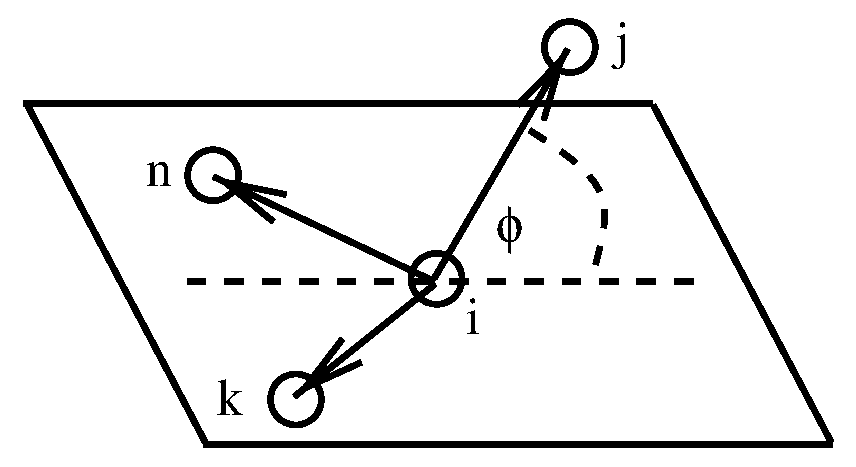
\includegraphics[height=4cm]{invers.eps}
\caption{The inversion angle and associated vectors}
\end{center}
\end{figure}

The inversion angle potentials\index{potential!inversion} describe the interaction arising from a
particular geometry of three atoms around a central atom. The best
known example of this is the arrangement of hydrogen atoms around
nitrogen in ammonia to form a trigonal pyramid. The hydrogens can
`flip' like an inverting umbrella to an alternative structure, which
in this case is identical, but in principle causes a change in
chirality. The force restraining the ammonia to one structure can be
described as an inversion potential\index{potential!inversion} (though it is usually augmented by
valence\index{potential!valence angle} angle potentials also). The inversion angle is defined in the
figure above - {\bf note that the inversion\index{potential!inversion} angle potential is a sum of
the three possible inversion\index{potential!inversion} angle terms.} It resembles a dihedral\index{potential!dihedral}
potential in that it requires the specification of four atomic
positions.

The potential functions available in \D{} are as
follows.
\begin{enumerate}
\item Harmonic: ({\bf harm})
\begin{equation}
U(\phi_{ijkn})= {1\over 2} k (\phi_{ijkn} - \phi_0)^2 
\end{equation}
\item Harmonic cosine: ({\bf hcos})
\begin{equation}
U(\phi_{ijkn})={k\over 2}(cos(\phi_{ijkn}) -cos(\phi_{0}))^{2}
\end{equation}
\item Planar potential: ({\bf plan})
\begin{equation}
U(\phi_{ijkn})= A \left [ 1 - \cos (\phi_{ijkn})\right] 
\end{equation}
\end{enumerate}
In these formulae $\phi_{ijkn}$ is the inversion\index{potential!inversion} angle defined by
\begin{equation}
\phi_{ijkn}=\cos^{-1}\left \{\frac{\vek{r}_{ij}\cdot\vek{w}_{kn}}{r_{ij}w_{kn}}\right \},
\end{equation}
with
\begin{equation}
\vek{w}_{kn}=(\vek{r}_{ij}\cdot\vek{\hat{u}}_{kn})\vek{\hat{u}}_{kn}+
(\vek{r}_{ij}\cdot\vek{\hat{v}}_{kn})\vek{\hat{v}}_{kn}
\end{equation}
and the unit vectors
\begin{eqnarray}
\vek{\hat{u}}_{kn}&=&(\vek{\hat{r}}_{ik}+\vek{\hat{r}}_{in})/
|\vek{\hat{r}}_{ik}+\vek{\hat{r}}_{in}| \nonumber  \\
\vek{\hat{v}}_{kn}&=&(\vek{\hat{r}}_{ik}-\vek{\hat{r}}_{in})/
|\vek{\hat{r}}_{ik}-\vek{\hat{r}}_{in}|.
\end{eqnarray}
As usual, $\vek{r}_{ij}=\vek{r}_{j}-\vek{r}_{i}$ {\em etc.} and the
hat $\vek{\hat{r}}$ indicates a {\em unit} vector in the direction of
$\vek{r}$. The total inversion\index{potential!inversion} potential requires the calculation of
three such angles, the formula being derived from the above using the
cyclic permutation of the indices $j\rightarrow k \rightarrow n
\rightarrow j$ {\em etc}.

Equivalently, the angle $\phi_{ijkn}$ may be written as
\begin{equation}
\phi_{ijkn}=\cos^{-1} \left \{ \frac{
[(\vek{r}_{ij}\cdot\vek{\hat{u}}_{kn})^{2}
+(\vek{r}_{ij}\cdot\vek{\hat{v}}_{kn})^{2}]^{1/2}}{r_{ij}}\right \}
\end{equation}

Formally, the force on an atom arising from the inversion\index{potential!inversion} potential is given by
\begin{equation}
f_{\ell}^{\alpha}=-\frac{\partial}{\partial
r_{\ell}^{\alpha}}U(\phi_{ijkn}),
\end{equation}
with $\ell$ being one of $i,j,k,n$ and $\alpha$ one of $x,y,z$. This
may be expanded into
\begin{eqnarray}
-\frac{\partial}{\partial r_{\ell}^{\alpha}}U(\phi_{ijkn})&=&
\left\{\frac{1}{\sin(\phi_{ijkn})}\right\}
\frac{\partial}{\partial \phi_{ijkn}}U(\phi_{ijkn})\times \nonumber \\
& & \frac{\partial}{\partial r_{\ell}^{\alpha}}
\left\{\frac{[(\vek{r}_{ij}\cdot\vek{\hat{u}}_{kn})^{2}
+(\vek{r}_{ij}\cdot\vek{\hat{v}}_{kn})^{2}]^{1/2}}
{r_{ij}}\right \}.
\end{eqnarray}
Following through the (extremely tedious!) differentiation gives the result:
\begin{eqnarray}
f_{\ell}^{\alpha} &=&
\left\{\frac{1}{\sin(\phi_{ijkn})}\right\}
\frac{\partial}{\partial \phi_{ijkn}}U(\phi_{ijkn})\times \\
& &
\left\{-(\delta_{\ell j}-\delta_{\ell i})\frac{cos(\phi_{ijkn})}
{r_{ij}^{2}}r_{ij}^{\alpha} +\frac{1}{r_{ij}w_{kn}}\left [
(\delta_{\ell j}-\delta_{\ell i}) 
\{(\vek{r}_{ij}\cdot\vek{\hat{u}}_{kn})\hat{u}_{kn}^{\alpha}+
(\vek{r}_{ij}\cdot\vek{\hat{v}}_{kn})\hat{v}_{kn}^{\alpha}\} 
\phantom{\left\{\frac{a_{a}^{a}}{a_{a}^{a}}\right\}}
\right. \right. \nonumber \\
& & + (\delta_{\ell k}-\delta_{\ell i})
\frac{\vek{r}_{ij}\cdot\vek{\hat{u}}_{kn}}{u_{kn}r_{ik}}\left \{
r_{ij}^{\alpha}-(\vek{r}_{ij}\cdot\vek{\hat{u}}_{kn})\hat{u}_{kn}^{\alpha}
-(\vek{r}_{ij}\cdot\vek{r}_{ik}-(\vek{r}_{ij}\cdot\vek{\hat{u}}_{kn})
(\vek{r}_{ik}\cdot\vek{\hat{u}}_{kn}))\frac{r_{ik}^{\alpha}}{r_{ik}^{2}}
\right \} \nonumber \\
& & + (\delta_{\ell k}-\delta_{\ell i})
\frac{\vek{r}_{ij}\cdot\vek{\hat{v}}_{kn}}{v_{kn}r_{ik}}\left \{
r_{ij}^{\alpha}-(\vek{r}_{ij}\cdot\vek{\hat{v}}_{kn})\hat{v}_{kn}^{\alpha}
-(\vek{r}_{ij}\cdot\vek{r}_{ik}-(\vek{r}_{ij}\cdot\vek{\hat{v}}_{kn})
(\vek{r}_{ik}\cdot\vek{\hat{v}}_{kn}))\frac{r_{ik}^{\alpha}}{r_{ik}^{2}}
\right \} \nonumber \\
& &+ (\delta_{\ell n}-\delta_{\ell i})
\frac{\vek{r}_{ij}\cdot\vek{\hat{u}}_{kn}}{u_{kn}r_{in}}\left \{
r_{ij}^{\alpha}-(\vek{r}_{ij}\cdot\vek{\hat{u}}_{kn})\hat{u}_{kn}^{\alpha}
-(\vek{r}_{ij}\cdot\vek{r}_{in}-(\vek{r}_{ij}\cdot\vek{\hat{u}}_{kn})
(\vek{r}_{in}\cdot\vek{\hat{u}}_{kn}))\frac{r_{in}^{\alpha}}{r_{in}^{2}}
\right \} \nonumber \\
& & \left . \left .- (\delta_{\ell n}-\delta_{\ell i})
\frac{\vek{r}_{ij}\cdot\vek{\hat{v}}_{kn}}{v_{kn}r_{in}}\left \{
r_{ij}^{\alpha}-(\vek{r}_{ij}\cdot\vek{\hat{v}}_{kn})\hat{v}_{kn}^{\alpha}
-(\vek{r}_{ij}\cdot\vek{r}_{in}-(\vek{r}_{ij}\cdot\vek{\hat{v}}_{kn})
(\vek{r}_{in}\cdot\vek{\hat{v}}_{kn}))\frac{r_{in}^{\alpha}}{r_{in}^{2}}
\right \} \right ] \right \} \nonumber 
\end{eqnarray}
This general formula applies to all atoms $\ell=i,j,k,n$. It must be
remembered however, that these formulae apply to just
one of the three contributing terms (i.e. one angle $\phi$) of the
full inversion\index{potential!inversion} potential: specifically the inversion\index{potential!inversion} angle pertaining
to the out-of-plane vector $\vek{r}_{ij}$. The contributions arising
from the other vectors $\vek{r}_{ik}$ and $\vek{r}_{in}$ are obtained
by the cyclic permutation of the indices in the manner described
above.  All these force contributions must be added to the final
atomic forces.

Formally, the contribution to be added to the
atomic virial is given by
\begin{equation}
{\cal W}=-\sum_{i=1}^{4}\vek{r}_{i}\cdot\vek{f}_{i}
\end{equation}

However it is possible to show by thermodynamic arguments ({\em cf}
\cite{smith-93c},) or simply from the fact that the sum of forces on
atoms j,k and n is equal and opposite to the force on atom i, that the
inversion potential makes\index{potential!inversion} {\em no} contribution to the atomic virial.

If the force components $f_{\ell}^{\alpha}$ for atoms $\ell=i,j,k,n$ are
calculated using the above formulae, it is easily seen that
the contribution to be added to the atomic stress tensor\index{stress tensor} is given by
\begin{equation}
\sigma^{\alpha \beta}=r_{ij}^{\alpha}f_{j}^{\beta}+
r_{ik}^{\alpha}f_{k}^{\beta}+r_{in}^{\alpha}f_{n}^{\beta}
\end{equation}
The sum of the diagonal elements of the stress tensor\index{stress tensor} is zero (since
the virial is zero) and the matrix is symmetric.

In \D{} inversion\index{potential!inversion} forces are handled by the routine {\sc invfrc}.

\subsection{The Calcite Four-Body Potential}
\label{calcite}
\begin{figure}[ht]
\begin{center}
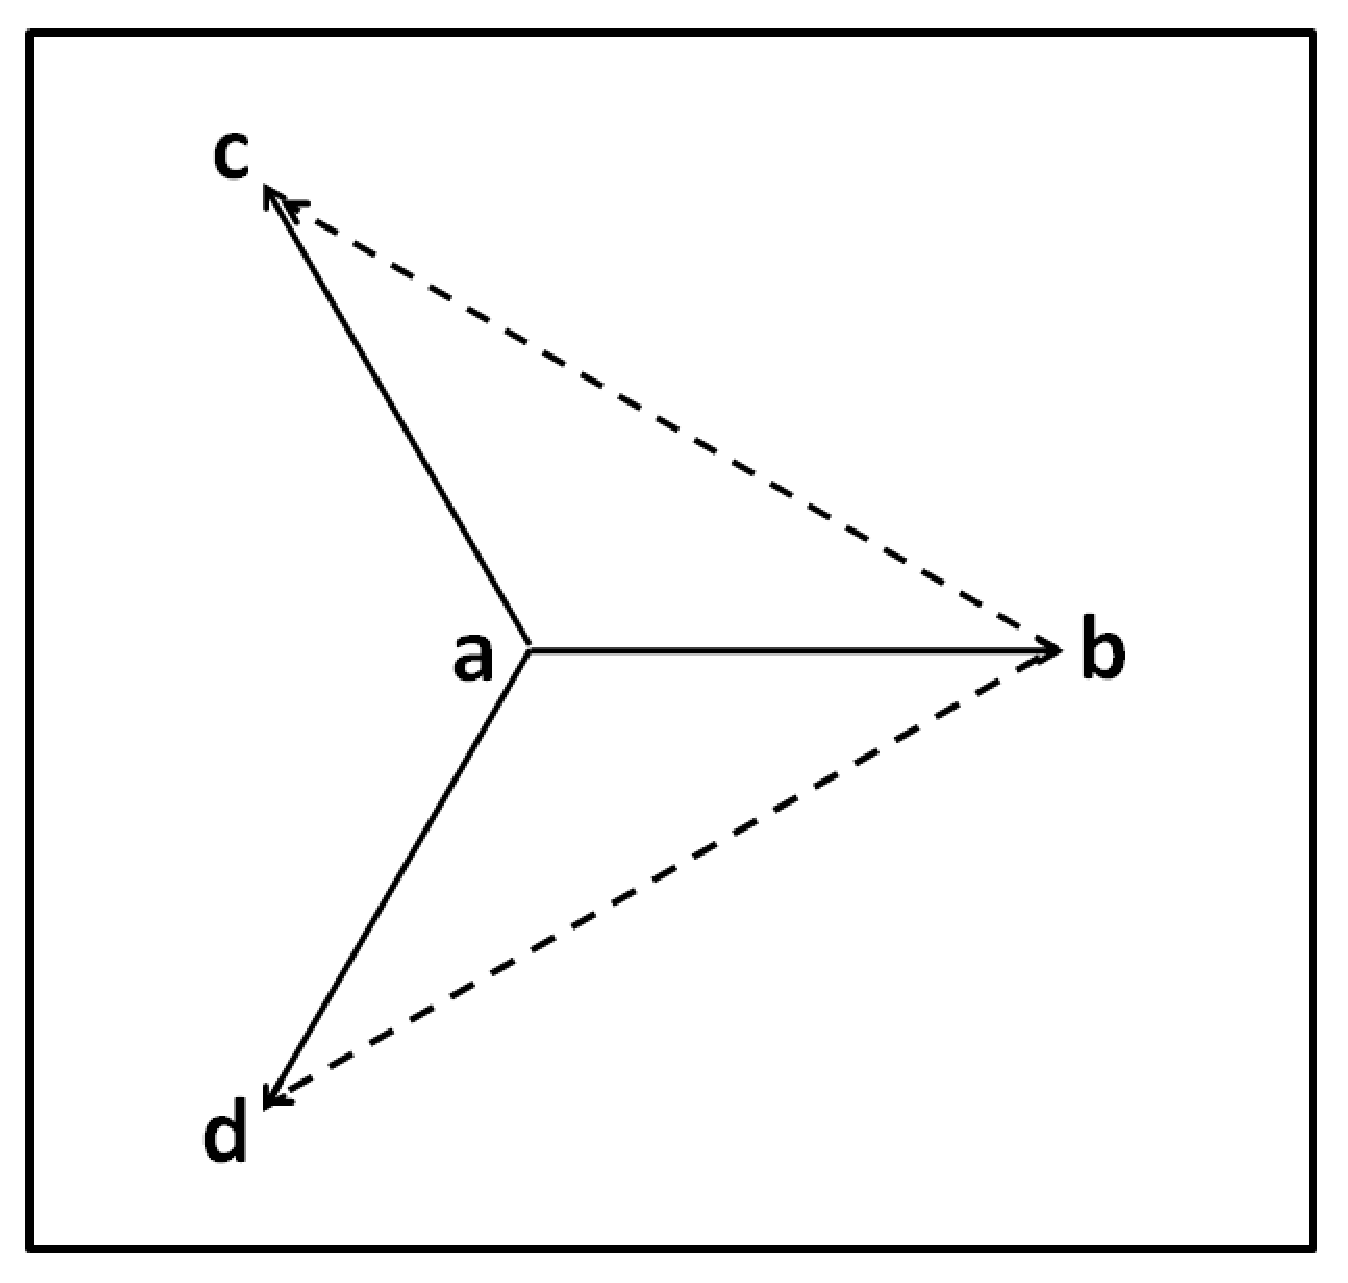
\includegraphics[height=4cm]{calcite.eps}
\caption{The vectors of the calcite potential}
\label{calcfig}
\end{center}
\end{figure}
\index{potential!calcite} This potential \cite{rohl-03a} is designed to help
maintain the planar structure of the carbonate anion $[CO_{3}]^{2-}$ in a
similar manner to the planar inversion potential described above. However it
is {\em not} an angular potential. It is dependent on the perpendicular
displacement ($u$) of an atom $a$ from a plane defined by three other atoms
$b$, $c$, and $d$ (see figure \ref{calcfig}) and has the form
\begin{equation}
U_{abcd}(u)=Au^{2}+Bu^{4} \label{calcite1}
\end{equation}
Where the displacement $u$ is given by
\begin{equation}
u=\frac{\vek{r}_{ab}\cdot\vek{r}_{bc}\times\vek{r}_{bd}}{|\vek{r}_{bc}\times\vek{r}_{bd}|}.\label{calcite2}
\end{equation}
Vectors $\vek{r}_{ab}$,$\vek{r}_{ac}$ and $\vek{r}_{ad}$ define bonds between
the central atom $a$ and the peripheral atoms $b$, $c$ and $d$. Vectors
$\vek{r}_{bc}$ and $\vek{r}_{bd}$ define the plane and are related to the bond
vectors by:
\begin{eqnarray}
\vek{r}_{bc}&=&\vek{r}_{ac}-\vek{r}_{ab} \nonumber \\
\vek{r}_{bd}&=&\vek{r}_{ad}-\vek{r}_{ab}.
\end{eqnarray}
It what follows it is convenient to define the vector product appearing in
both the numerator and denominator of equation (\ref{calcite2}) as the vector
$\vek{w}_{cd}$ {\em vis.}
\begin{equation}
\vek{w}_{cd}=\vek{r}_{bc}\times\vek{r}_{bd}
\end{equation}
We also define the quantity $\gamma(u)$ as
\begin{equation}
\gamma(u)=-(2Au+4Bu^{3}).
\end{equation}
The forces on the individual atoms due to the calcite potential are then given
by 
\begin{eqnarray}
\vek{f}_{a}&=&-\gamma(u)\hat{\vek{w}}_{cd} \nonumber \\
\vek{f}_{c}&=&\phantom{+}\vek{r}_{bd}\times(\vek{r}_{ab}-
u\hat{\vek{w}}_{cd})\gamma(u)/w_{cd} \nonumber \\
\vek{f}_{d}&=&-\vek{r}_{bc}\times(\vek{r}_{ab}-
u\hat{\vek{w}}_{cd})\gamma(u)/w_{cd} \nonumber \\
\vek{f}_{b}&=&-(\vek{f}_{a}+\vek{f}_{c}+\vek{f}_{d}),
\end{eqnarray}
where $w_{cd}=|\vek{w}_{cd}|$ and $\hat{\vek{w}}_{cd}=\vek{w}_{cd}/w_{cd}$.
The virial contribution $\psi_{abcd}(u)$ is given by
\begin{equation}
\psi_{abcd}(u)=2Au^{2}+4Bu^{4}
\end{equation}
and the stress tensor contribution $\sigma_{abcd}^{\alpha\beta}(u)$ by
\begin{equation}
\sigma_{abcd}^{\alpha\beta}(u)=\frac{u\gamma(u)}{
  w_{cd}^{2}}w_{cd}^{\alpha}w_{cd}^{\beta}.
\end{equation}

In \D{} the calcite\index{potential!calcite} forces are handled by the routine
{\sc invfrc}, which is a convenient {\em intramolecular} four-body force
routine. However it is manifestly {\em not} an inversion potential as such.

\subsection{Tethering Forces}

\D{} also allows atomic sites to be tethered\index{potential!tethered} to a fixed point in space, $\vek{r}_0$ taken as their
position at the beginning of the simulation. This is also known as position restraining.
The specification, which comes as part of the molecular description,
requires a tether\index{potential!tethered} potential type and the associated interaction parameters.

Note, firstly, that application of tethering\index{potential!tethered} potentials means that momentum will
no longer be a conserved quantity of the simulation. Secondly, in constant
pressure simulations, where the MD cell changes size or shape, the reference position
is scaled with the cell vectors.

The potential functions available in \D{} are as
follows, in each case $r_{i0}$ is the distance of the atom from its position at $t=0$:
\begin{enumerate}
\item harmonic potential: ({\bf harm})
\begin{equation}
U(r_{i0}) = \frac{1}{2}k(r_{i0})^2;
\end{equation}
\item restrained harmonic :({\bf rhrm})
\begin{eqnarray}
U(r_{i0})&=&\frac{1}{2}k(r_{i0})^2~~~~~~r_{i0}\le r_{c};\\
U(r_{i0})&=&\frac{1}{2}kr_{c}^2+kr_{c}(r_{i0}-r_{c})~~~~~~r_{i0}>r_{c};
\end{eqnarray}
\item Quartic potential: ({\bf quar})
\begin{equation}
U(r_{i0})=\frac{k}{2}(r_{i0})^2+\frac{k'}{3}(r_{i0})^3+\frac{k''}{4}(r_{i0})^4.
\end{equation}
\end{enumerate}

The force on the atom $i$ arising from a tether\index{potential!tethered} potential is obtained
using the general formula:
\begin{equation}
\vek{f}_{i}=-\frac{1}{r_{i0}}\left[
\frac{\partial }{\partial r_{i0}}U(r_{i0})\right]\vek{r}_{i0},
\end{equation}

The contribution to be added to the atomic virial is given by
\begin{equation}
{\cal W}=\vek{r}_{i0}\cdot \vek{f}_{i},
\end{equation}

The contribution to be added to the atomic stress tensor\index{stress tensor} is
given by
\begin{equation}
\sigma^{\alpha \beta}=-r_{i0}^{\alpha}f_{i}^{\beta},
\end{equation}
where $\alpha$ and $\beta$ indicate the $x,y,z$ components. The atomic
stress tensor\index{stress tensor} derived in this way is symmetric.

In \D{} bond\index{potential!bond} forces are handled by the routine {\sc tethfrc}.

\subsection{Frozen Atoms}
\D{} also allows atoms to be completely immobilised ({\em i.e.}
``frozen'' at a fixed point in the MD cell). This is achieved by
setting all forces and velocities associated with that atom to zero
during each MD timestep.  Frozen atoms are signalled by assigning an
atom a non-zero value for the freeze parameter in the FIELD file.  \D{}
does not calculate contributions to the virial or the stress
tensor\index{stress tensor}
arising from the constraints required to freeze atomic positions. In
\D{} the frozen atom option cannot be used for sites in a rigid
body\index{rigid body}. As with the tethering\index{potential!tethered} potential, the reference position is scaled with
the cell vectors in constant pressure simulations.

In \D{} the frozen atom option is handled by the subroutine {\sc freeze}.


\section{The Intermolecular Potential Functions}
\label{intermolecular}
In this section we outline the pair-body, three-body\index{potential!three-body} and four-body\index{potential!four-body}
potential functions available in \D{}. An important distinction between
these and intramolecular\index{potential!intramolecular} (bond) forces in \D{} is that they are
specified by {\em atom types} rather than atom indices.

\subsection{Short Ranged (van der Waals) Potentials}
\label{vdwpot}

The short ranged pair forces available in \D{} are as
follows.

\begin{enumerate}
\item 12 - 6 potential: ({\bf 12-6})
\begin{equation}
U(r_{ij})=\left(\frac{A}{r_{ij}^{12}}\right)-\left(\frac{B}{r_{ij}^{6}}\right);
\end{equation}
\item Lennard-Jones: ({\bf lj})
\begin{equation}
U(r_{ij})=4\epsilon\left[\left
(\frac{\sigma}{r_{ij}}\right)^{12}-\left(\frac{\sigma}{r_{ij}}\right)^{6}\right
];
\end{equation}
\item n - m potential \cite{clarke-86a}: ({\bf nm})
\begin{equation}
U(r_{ij})=\frac{E_{o}}{(n-m)}\left[m\left 
(\frac{r_{o}}{r_{ij}}\right)^{n}-n\left(\frac{r_{o}}{r_{ij}}\right)^{m}\right
];
\end{equation}
\item Buckingham potential: ({\bf buck})
\begin{equation}
U(r_{ij})=A~\exp\left(-\frac{r_{ij}}{\rho}\right)-\frac{C}{r_{ij}^{6}};
\end{equation}
\item Born-Huggins-Meyer potential: ({\bf bhm})
\begin{equation}
U(r_{ij})=A~\exp[B(\sigma-r_{ij})]-\frac{C}{r_{ij}^{6}}-\frac{D}{r_{ij}^{8}};
\end{equation}
\item Hydrogen-bond (12 - 10) potential: ({\bf hbnd})
\begin{equation}
U(r_{ij})=\left(\frac{A}{r_{ij}^{12}}\right)-\left(\frac{B}{r_{ij}^{10}}\right);
\end{equation}
\item Shifted force n - m potential \cite{clarke-86a}: ({\bf snm})
\begin{eqnarray}
U(r_{ij})&=&\frac{\alpha E_{o}}{(n-m)}\left [
m\beta^{n}\left \{ \left (\frac{r_{o}}{r_{ij}}\right )^{n}-
\left(\frac{1}{\gamma}\right)^{n}\right \}-
n\beta^{m}\left \{ \left (\frac{r_{o}}{r_{ij}}\right )^{m}-
\left(\frac{1}{\gamma}\right)^{m}\right \} \right ]\nonumber \\
& & +\frac{nm\alpha E_{o}}{(n-m)} \left ( \frac{r_{ij}-\gamma r_{o}}{\gamma r_{o}}
\right )\left\{\left(\frac{\beta}{\gamma}\right
)^{n}-\left(\frac{\beta}{\gamma}\right )^{m}\right \}
\end{eqnarray}
with
\begin{eqnarray}
\gamma &=&\frac{r_{cut}}{r_{o}} \\
\beta &=& \gamma\left ( \frac{\gamma^{m+1}-1}{\gamma^{n+1}-1} \right )
^{\frac{1}{n-m}} \\
\alpha&=&\frac{(n-m)}{[n\beta^{m}(1+(m/\gamma-m-1)/\gamma^{m})-
m\beta^{n}(1+(n/\gamma-n-1)/\gamma^{n})]}
\end{eqnarray}
This peculiar form has the advantage over the standard shifted n-m
potential in that both $E_{o}$ and $r_{0}$ (well depth and location of
minimum) retain their original values after the shifting process.
\item Morse potential:  ({\bf mors})
\begin{equation}
U(r_{ij})=E_{o}[\{1-\exp(-k(r_{ij}-r_{o}))\}^{2}-1];
\end{equation}
\item Shifted Weeks-Chandler-Anderson (WCA) potential \cite{weeks-71}:  ({\bf wca})
\begin{equation}
U(r_{ij}) = \left\{ \begin{array} {l@{\qquad:\qquad}l}
4\epsilon\left[\left(\frac{\sigma}{r_{ij}-\Delta}\right)^{12}-\left(\frac{\sigma}{r_{ij}-\Delta}\right)^{6}\right]
+\epsilon & r_{ij} < 2^{1 \over 6}~\sigma + \Delta \\
0 & r_{ij} \ge 2^{1 \over 6}~\sigma + \Delta \end{array} \right. \label{wca}
\end{equation}
The WCA potential is the Lennard-Jones potential truncated at the
position of the minimum and shifted to eliminate discontinuity
(includes the effect of excluded volume).  It is usually used in
combination with the FENE (\ref{FENE}) bond potential.  This
implementation allows for a radius shift of up to half a $\sigma$
($|\Delta| \le 0.5~\sigma$) with a default of zero
($\Delta_{default} = 0$).

\item Gaussian potential ({\bf gaus})
\begin{equation}
U(r_{ij}) = \sum_{n}^{3} A_{n}exp(-b_{b}r_{ij}^{2})
\end{equation}
Up to 3 Gaussian terms are permitted, unrequired terms have $A_{n}=0$.

\item Tabulation: ({\bf tab}). The potential is defined numerically only.
\end{enumerate}

The parameters defining these potentials are supplied to
\D{} at run time (see the description of the FIELD file in section
\ref{fieldfile}). Each atom type in the system is specified by a unique
eight-character label defined by the user. The pair potential is then
defined internally by the combination of two atom labels.

As well as the numerical parameters defining the potentials,
\D{} must also be provided with a cutoff radius $r_{cut}$,
which sets a ranged limit on the computation of the interaction.
Together with the parameters, the cutoff is used by the subroutine
{\sc forgen} (or {\sc forgen\_rsq}) to construct an interpolation
array {\tt vvv} for the potential function over the ranged 0 to
$r_{cut}$. A second array {\tt ggg} is also calculated, which is
related to the potential via the formula:
\begin{equation}
G(r_{ij})=-r_{ij}\frac{\partial}{\partial r_{ij}}U(r_{ij}),
\end{equation}
and is used in the calculation of the forces. Both arrays are
tabulated in units of energy.  The use of interpolation arrays, rather
than the explicit formulae, makes the routines for calculating the
potential energy and atomic forces very general, and
enables the use of user defined pair potential functions.
\D{} also allows the user to read in the interpolation arrays
directly from a file (see the description of the TABLE file (section
\ref{tablefile}).  This is particularly useful if the pair potential
function has no simple analytical description (e.g.  spline
potentials).

The force on an atom $j$ derived from one of these potentials is
formally calculated with the standard formula:
\begin{equation}
\vek{f}_{j}=-\frac{1}{r_{ij}}\left[\frac{\partial}{\partial 
r_{ij}}U(r_{ij})\right]\vek{r}_{ij},
\end{equation}
where $\vek{r}_{ij}=\vek{r}_{j}-\vek{r}_{i}$. The force on atom $i$ is
the negative of this.

The contribution to be added to the atomic virial (for each pair
interaction) is
\begin{equation}
{\cal W}=-\vek{r}_{ij}\cdot\vek{f}_{j}.
\end{equation}

The contribution to be added to the atomic stress tensor\index{stress tensor} is
given by
\begin{equation}
\sigma^{\alpha \beta}=r_{ij}^{\alpha}f_{j}^{\beta},
\end{equation}
where $\alpha$ and $\beta$ indicate the $x,y,z$ components. The atomic
stress tensor\index{stress tensor} derived from the pair forces is symmetric.

Since the calculation of pair potentials assumes a spherical cutoff
($r_{cut}$) it is necessary to apply a {\em long ranged
correction}\index{long ranged corrections!van der Waals} to
the system potential energy and virial. Explicit formulae are needed
for each case and are derived as follows. For two atom types $a$ and
$b$, the correction for the potential energy is calculated via the
integral
\begin{equation}
U_{corr}^{ab}=2\pi
\frac{N_{a}N_{b}}{V}\int_{r_{cut}}^{\infty}g_{ab}(r)U_{ab}(r)r^{2}dr
\end{equation}
where $N_{a},N_{b}$ are the numbers of atoms of types $a$ and $b$, $V$
is the system volume and $g_{ab}(r)$ and $U_{ab}(r)$ are the
appropriate pair correlation function and pair potential respectively.
It is usual to assume $g_{ab}(r)=1$ for $r>r_{cut}$. \D{}
sometimes makes the additional assumption that the repulsive part of
the short ranged potential is negligible beyond $r_{cut}$. 

The correction for the system virial is
\begin{equation}
{\cal W}_{corr}^{ab}=-2\pi
\frac{N_{a}N_{b}}{V}\int_{r_{cut}}^{\infty}g_{ab}(r)\frac{\partial}{\partial
r}U_{ab}(r)r^{3}dr,
\end{equation}
where the same approximations are applied. Note that these formulae
are based on the assumption that the system is reasonably isotropic
beyond the cutoff.

In \D{} the short ranged forces are calculated by one of the
routines {\sc srfrce, srfrce\_rsq,} and {\sc srfrceneu}. The long
ranged corrections are calculated by routine {\sc lrcorrect}. The
calculation makes use of the Verlet\index{algorithm!Verlet} neighbour list described above.

\subsection{Three Body Potentials}

The three-body\index{potential!three-body} potentials in \D{} are mostly
valence angle\index{potential!valence angle} forms. (They are
primarily included to permit simulation of amorphous materials
e.g. silicate glasses.) However, these have been extended to include
the Dreiding\index{force field!Dreiding} \cite{mayo-90a} hydrogen
bond. The potential forms available are as follows.

\begin{enumerate}
\item Harmonic: ({\bf harm})
\begin{equation}
U(\theta_{jik})= {k\over 2} (\theta_{jik} - \theta_0)^2
\end{equation}
\item Truncated harmonic: ({\bf thrm})
\begin{equation}
U(\theta_{jik})= {k\over 2} (\theta_{jik} - \theta_0)^2
\exp[-(r_{ij}^8 + r_{ik}^8)/\rho^8];
\end{equation}
\item Screened Harmonic: ({\bf shrm})
\begin{equation}
 U(\theta_{jik})= {k\over 2} (\theta_{jik} - \theta_0)^2
\exp[-(r_{ij}/\rho_1 + r_{ik}/\rho_2)] ;
\end{equation}
\item Screened Vessal\cite{vessal-94a}: ({\bf bvs1})
\begin{eqnarray}
U(\theta_{jik})&=& {k \over 8(\theta_{jik}-\pi)^2}\left\{ \left[
(\theta_0 -\pi)^2 -(\theta_{jik}-\pi)^2\right]^2
\right\} \nonumber \\
& & \exp[-(r_{ij}/\rho_1 + r_{ik}/\rho_2)];
\end{eqnarray}
\item Truncated Vessal\cite{smith-95a}: ({\bf bvs2})
\begin{eqnarray}
 U(\theta_{jik})&=& k\big[ \theta_{jik}^a (\theta_{jik}-\theta_0)^2
(\theta_{jik}+\theta_0-2\pi)^2  - {a\over 2} \pi^{a-1}\nonumber \\
& & (\theta_{jik}-\theta_0)^2(\pi - \theta_0)^3\big]
\exp[-(r_{ij}^8 + r_{ik}^8)/\rho^8].
\end{eqnarray}
\item Dreiding\index{force field!Dreiding} hydrogen bond \cite{mayo-90a}:
({\bf hbnd})
 \begin{equation}
U(\theta_{jik})=D_{hb}cos^{4}(\theta_{jik})[5(R_{hb}/r_{jk})^{12}-6(R_{hb}/r_{jk})^{10}]
\end{equation}
\end{enumerate}
Note that for the hydrogen bond\index{potential!bond}, the hydrogen atom {\em must} be the
central atom.  Several of these functions are identical to those
appearing in the {\em intra-}molecular valence\index{potential!valence
angle}angle descriptions
above. There are significant differences in implementation however,
arising from the fact that the three-body\index{potential!three-body} potentials are regarded as
{\em inter-}molecular.  Firstly, the atoms involved are defined by
atom types, not specific indices.  Secondly, there are {\em no}
excluded atoms arising from the three body terms\index{potential!three-body}. (The inclusion of
pair potentials may in fact be essential to maintain the structure of
the system.)

The three body\index{potential!three-body} potentials are very short
ranged, typically of order 3~$\AA$. This property, plus the fact that
three body\index{potential!three-body} potentials scale as $N^{3}$,
where $N$ is the number of particles, makes it essential that these
terms are calculated by the link-cell method \cite{eastwood-80a}.

The calculation of the forces, virial and stress tensor\index{stress tensor} as
described in the section valence angle\index{potential!valence angle} potentials above.

\D{} applies no long ranged corrections to the three body\index{potential!three-body} potentials.
The three body\index{potential!three-body} forces are calculated by the routine {\sc thbfrc}.

\subsection{The Tersoff Covalent Potential}
\label{tersoff}

The Tersoff\index{potential!Tersoff} potential \cite{tersoff-89a} is a
special example of a density dependent potential, which has been
designed to reproduce the properties of covalent bonding in systems
containing carbon, silicon, germanium etc and alloys of these
elements.  
A special feature of the potential is that it allows bond breaking and
associated changes in bond hybridisation.
The potential has 11 atomic and 2 bi-atomic parameters.  The energy is
modelled as a sum of pair-like interactions where, however, the
coefficient of the attractive term in the pairlike potential (which
plays the role of a bond order) depends on the local environment
giving a many-body potential.

The form of the Tersoff potential is:  ({\bf ters})
\begin{equation}
U_{ij} = f_{C}(r_{ij})~[f_{R}(r_{ij}) - \gamma_{ij}~f_{A}(r_{ij})],
\end{equation}
where
\begin{equation}
f_{R}(r_{ij}) = A_{ij}~\exp(- a_{ij}~r_{ij})~,~~
f_{A}(r_{ij}) = B_{ij}~\exp(- b_{ij}~r_{ij})
\end{equation}
\begin{equation}
f_{C}(r_{ij}) = \left\{ \begin{array} {l@{\qquad:\qquad}l}
1 & r_{ij} < R_{ij} \\
\frac{1}{2} + \frac{1}{2} \cos [\pi~(r_{ij}-R_{ij})/(S_{ij}-R_{ij})] & R_{ij} < r_{ij} < S_{ij} \\
0 & r_{ij} > S_{ij}
\end{array} \right.
\end{equation}
\begin{eqnarray}
\gamma_{ij} = \chi_{ij}~(1 + {\beta_{i}}^{\eta_{i}}~{\cal{L}}_{ij}^{\eta_{i}})^{-1/2\eta_{i}}~,~~
{\cal{L}}_{ij} = \sum_{k \neq i,j} f_{C}(r_{ik})~\omega_{ik}~g(\theta_{ijk}) \nonumber \\
g(\theta_{ijk}) = 1 + c_{i}^2/d_{i}^2 - c_{i}^2/[d_{i}^2 + (h_{i} - \cos\theta_{ijk})^2]
\end{eqnarray}
with further mixed parameters defined as
\begin{eqnarray}
a_{ij} = (a_{i} + a_{j})/2&,&~b_{ij} = (b_{i} + b_{j})/2 \nonumber \\
A_{ij} = (A_{i} A_{j})^{1/2}&,&~B_{ij} = (B_{i} B_{j})^{1/2} \\
R_{ij} = (R_{i} R_{j})^{1/2}&,&~S_{ij} = (S_{i} S_{j})^{1/2}~~.
\nonumber
\end{eqnarray}
Here $i,~j$ and $k$ label the atoms in the system, $r_{ij}$ is the
length of the $ij$ bond, and $\theta_{ijk}$ is the bond angle between
bonds $ij$ and $ik$.  Single subscripted parameters (11), such as
$a_{i}$ and $\eta_{i}$, depend only on the type of atom.

The chemistry between different atom types is encapsulated in the two
sets of bi-atomic parameters $\chi_{ij}$ and $\omega_{ij}$:
\begin{eqnarray}
\chi_{ii}~=~1&,&~\chi_{ij}~=~\chi_{ji} \nonumber \\
\omega_{ii}~=~1&,&~\omega_{ij}~=~\omega_{ji}~~,
\end{eqnarray}
which define only one independent parameter for each pair of atom
types.  The $\chi$ parameter is used to strengthen or weaken the
heteropolar bonds, relative to the value obtained by simple
interpolation.  The $\omega$ parameter is used to permit greater
flexibility when dealing with more drastically different types of
atoms.

The force on an atom $\ell$ derived from this potential is
formally calculated with the formula:
\begin{equation}
f_{\ell}^{\alpha} = -\frac{\partial}{\partial r_{\ell}^{\alpha}}
E_{\tt tersoff} = \frac{1}{2} \sum_{i \neq j}
-\frac{\partial}{\partial r_{\ell}^{\alpha}} U_{ij}~~,
\end{equation}
with atomic label $\ell$ being one of $i,j,k$ and $\alpha$
indicating the $x,y,z$ component.  The derivative in the above formula
expands into
\begin{equation}
-\frac{\partial U_{ij}}{\partial r_{\ell}^{\alpha}} =
-\frac{\partial}{\partial r_{\ell}^{\alpha}} f_{C}(r_{ij}) f_{R}(r_{ij}) +
 \gamma_{ij} \frac{\partial}{\partial r_{\ell}^{\alpha}} f_{C}(r_{ij}) f_{A}(r_{ij}) +
 f_{C}(r_{ij}) f_{A}(r_{ij}) \frac{\partial}{\partial r_{\ell}^{\alpha}} \gamma_{ij}~~,
\end{equation}
with the contributions from the first two terms being:
\begin{eqnarray}
-\frac{\partial}{\partial r_{\ell}^{\alpha}} f_{C}(r_{ij}) f_{R}(r_{ij})&=&
-\left\{ f_{C}(r_{ij}) \frac{\partial}{\partial r_{ij}} f_{R}(r_{ij}) +
f_{R}(r_{ij}) \frac{\partial}{\partial r_{ij}} f_{C}(r_{ij}) \right\} \times \nonumber \\
& & ~~\left\{ \delta_{j \ell} \frac{r_{i \ell}^{\alpha}}{r_{i \ell}} -
\delta_{i \ell} \frac{r_{\ell j}^{\alpha}}{r_{\ell j}} \right\}
\end{eqnarray}
\begin{eqnarray}
\gamma_{ij} \frac{\partial}{\partial r_{\ell}^{\alpha}} f_{C}(r_{ij}) f_{A}(r_{ij})&=&
\gamma_{ij} \left\{ f_{C}(r_{ij}) \frac{\partial}{\partial r_{ij}} f_{A}(r_{ij}) +
f_{A}(r_{ij}) \frac{\partial}{\partial r_{ij}} f_{C}(r_{ij}) \right\} \times \nonumber \\
& & ~~~\left\{ \delta_{j \ell} \frac{r_{i \ell}^{\alpha}}{r_{i \ell}} -
\delta_{i \ell} \frac{r_{\ell j}^{\alpha}}{r_{\ell j}} \right\}~~,
\end{eqnarray}
and from the third (angular) term:
\begin{eqnarray}
f_{C}(r_{ij}) f_{A}(r_{ij}) \frac{\partial}{\partial r_{\ell}^{\alpha}} \gamma_{ij}&=&
f_{C}(r_{ij}) f_{A}(r_{ij})~\chi_{ij}~~\times ~~~~~~~~~~~~~~~~~~~~~~~~~~ \nonumber \\
& & \left( -\frac{1}{2} \right) \left( 1 + {\beta_{i}}^{\eta_{i}}~{\cal{L}}_{ij}^{\eta_{i}}
\right)^{-\frac{1}{2 \eta_{i}} - 1} {\beta_{i}}^{\eta_{i}}~{\cal{L}}_{ij}^{\eta_{i}-1}
\frac{\partial}{\partial r_{\ell}^{\alpha}} {\cal{L}}_{ij}~~,
\end{eqnarray}
where
\begin{equation}
\frac{\partial}{\partial r_{\ell}^{\alpha}} {\cal{L}}_{ij} =
\frac{\partial}{\partial r_{\ell}^{\alpha}} \sum_{k \neq i,j}
\omega_{ik}~f_{C}(r_{ik})~g(\theta_{ijk})~~.  \nonumber
\end{equation}
The angular term can have three different contributions depending
on the index of the particle participating in the interaction:
\begin{eqnarray}
\ell~=~i~&:&~\frac{\partial}{\partial r_{i}^{\alpha}} {\cal{L}}_{ij} = \sum_{k \neq i,j} \omega_{ik}
\left[ g(\theta_{ijk}) \frac{\partial}{\partial r_{i}^{\alpha}} f_{C}(r_{ik}) +
f_{C}(r_{ik}) \frac{\partial}{\partial r_{i}^{\alpha}} g(\theta_{ijk}) \right]~~~~~~\\
\ell~=~j~&:&~\frac{\partial}{\partial r_{j}^{\alpha}} {\cal{L}}_{ij} = \sum_{k \neq i,j} \omega_{ik}
~f_{C}(r_{ik}) \frac{\partial}{\partial r_{j}^{\alpha}} g(\theta_{ijk}) \\
\ell~\neq~i,j~&:&~\frac{\partial}{\partial r_{\ell}^{\alpha}} {\cal{L}}_{ij} = \omega_{i \ell}
\left[ g(\theta_{ij \ell}) \frac{\partial}{\partial r_{\ell}^{\alpha}} f_{C}(r_{i \ell}) +
f_{C}(r_{i \ell}) \frac{\partial}{\partial r_{\ell}^{\alpha}} g(\theta_{ij \ell}) \right]~~.
\end{eqnarray}
The derivative of $g(\theta_{ijk})$ is worked out in the following
manner:
\begin{equation}
\frac{\partial}{\partial r_{\ell}^{\alpha}} g(\theta_{ijk}) =
\frac{\partial g(\theta_{ijk})}{\partial \theta_{ijk}}~
\frac{-1}{\sin \theta_{ijk}}~\frac{\partial}{\partial r_{\ell}^{\alpha}}
\left\{ \frac{\vek{r}_{ij} \cdot \vek{r}_{ik}} {r_{ij}~r_{ik}} \right\}~~,
\end{equation}
where
\begin{eqnarray}
\frac{\partial g(\theta_{ijk})}{\partial \theta_{ijk}}&=&
\frac{2~c_{i}^2(h_{i} - \cos \theta_{ijk})~\sin \theta_{ijk}}
{[d_{i}^2 + (h_{i} - \cos \theta_{ijk})^2]^2} \\
\frac{\partial}{\partial r_{\ell}^{\alpha}}
\left\{\frac{\vek{r}_{ij}\cdot\vek{r}_{ik}}{r_{ij}r_{ik}}\right\}&=&
(\delta_{\ell j}-\delta_{\ell i})\frac{r_{ik}^{\alpha}}{r_{ij}r_{ik}} +
(\delta_{\ell k}-\delta_{\ell i})\frac{r_{ij}^{\alpha}}{r_{ij}r_{ik}} - \nonumber \\
& & \cos(\theta_{jik}) \left\{(\delta_{\ell j}-\delta_{\ell i})\frac{r_{ij}^{\alpha}}{r_{ij}^{2}}+
(\delta_{\ell k}-\delta_{\ell i})\frac{r_{ik}^{\alpha}}{r_{ik}^{2}}\right\}~~.
\end{eqnarray}

The contribution to be added to the atomic virial can be derived
as
\begin{eqnarray}
{\cal W} &=& 3V \frac{\partial E_{\tt tersoff}}{\partial V} =
\frac{3~V}{2} \sum_{i \neq j} \frac{\partial U_{ij}}{\partial V} \\
{\cal W} &=& \frac{1}{2} \sum_{i} \sum_{j \neq i} \left\{ \left[
\frac{\partial}{\partial r_{ij}} f_{C}(r_{ij}) f_{R}(r_{ij}) -
\gamma_{ij} \frac{\partial}{\partial r_{ij}} f_{C}(r_{ij}) f_{A}(r_{ij})
\right] r_{ij} - \right.~~~~\nonumber \\
& & ~~~~\left( -\frac{1}{2} \right) f_{C}(r_{ij}) f_{A}(r_{ij})~\chi_{ij}
\left( 1 + {\beta_{i}}^{\eta_{i}}~{\cal{L}}_{ij}^{\eta_{i}} \right)^{-\frac{1}{2 \eta_{i}} - 1}
{\beta_{i}}^{\eta_{i}}~{\cal{L}}_{ij}^{\eta_{i}-1} \times \\
& & \left. ~~~~\sum_{k \neq i,j} \omega_{ik}~g(\theta_{ijk}) \left[
\frac{\partial}{\partial r_{ik}} f_{C}(r_{ik}) \right] r_{ik}~~ \right\}.
\nonumber
\end{eqnarray}

The contribution to be added to the atomic stress
tensor\index{stress tensor} is given by
\begin{equation}
\sigma^{\alpha \beta} = -r_{i}^{\alpha} f_{i}^{\beta}~~,
\end{equation}
where $\alpha$ and $\beta$ indicate the $x,y,z$ components.  The
stress tensor\index{stress tensor} is symmetric.

Interpolation arrays, {\tt vmbp} and {\tt gmbp} (set up in subroutine
{\sc tergen}) - similar to those in van der Waals
interactions \ref{vdwpot} - are used in the calculation of the Tersoff
forces, virial and stress.

The Tersoff\index{potential!Tersoff} potentials are very short
ranged, typically of order $3$~\AA.  This property, plus the fact
that Tersoff\index{potential!Tersoff} potentials (two- and
three-body contributions) scale as $N^{3}$, where $N$ is the number
of particles, makes it essential that these terms are calculated by
the link-cell method \cite{eastwood-80a}.

\D{} applies no long ranged corrections to the
Tersoff\index{potential!Tersoff} potentials.  In \D{} Tersoff forces
are handled by the routines {\sc tersoff, terint} and {\sc tersoff3}.

\subsection{Four Body Potentials}

The four-body\index{potential!four-body} potentials in \D{} are entirely inversion\index{potential!inversion} angle forms,
primarily included to permit simulation of amorphous materials
(particularly borate glasses). The potential forms available in \D{} are
as follows.
\begin{enumerate}
\item Harmonic: ({\bf harm})
\begin{equation}
U(\phi_{ijkn})= {1\over 2} k (\phi_{ijkn} - \phi_0)^2 
\end{equation}
\item Harmonic cosine: ({\bf hcos})
\begin{equation}
U(\phi_{ijkn})={k\over 2}(cos(\phi_{ijkn}) -cos(\phi_{0}))^{2}
\end{equation}
\item Planar potential: ({\bf plan})
\begin{equation}
U(\phi_{ijkn})= A  [ 1 - \cos (\phi_{ijkn})] 
\end{equation}
\end{enumerate}
These functions are identical to those appearing in the {\em
intra-}molecular\index{potential!intramolecular} inversion angle descriptions above. There are
significant differences in implementation however, arising from the
fact that the four-body\index{potential!four-body} potentials are regarded as {\em
inter-}molecular.  Firstly, the atoms involved are defined by atom
types, not specific indices.  Secondly, there are {\em no} excluded
atoms arising from the four-body\index{potential!four-body} terms. (The inclusion of other
potentials, for example pair potentials, may in fact be essential to
maintain the structure of the system.)

The four body\index{potential!four-body} potentials are very short
ranged, typically of order 3~$\AA$. This property, plus the fact that
four body\index{potential!four-body} potentials scale as $N^{4}$,
where $N$ is the number of particles, makes it essential that these
terms are calculated by the link-cell method \cite{eastwood-80a}.

The calculation of the forces, virial and stress tensor\index{stress tensor}
described in the section on inversion angle\index{potential!inversion} potentials above.

\D{} applies no long ranged corrections to the four body\index{potential!four-body} potentials.
The four-body\index{potential!four-body} forces are calculated by the routine {\sc fbpfrc}.

\subsection{Metal Potentials}
\label{metals}

The metal potentials in \D{} follow two similar but distinct formalisms.
The first of these is the embedded atom model (EAM)
\index{potential!embedded atom (EAM)} 
\index{embedded atom potential|see{potential,embedded atom (EAM)}}
\cite{baskes-84a,baskes-86a} and the second is the Finnis-Sinclair
model (FSM) \index{potential!Finnis-Sinclair} 
\index{Finnis-Sinclair potential|see{potential,Finnis-Sinclair}}
\cite{finnis-84a}. Both are density dependent potentials
derived from density functional theory (DFT) and describe the bonding
of a metal atom ultimately in terms of the local electronic density.
They are suitable for calculating the properties of metals
\index{potential!metal} and metal alloys.

For single component metals the two approaches are the same.  {\bf
However} they are subtly different in the way they are extended to
handle alloys (see below). It follows that EAM and FSM potentials
cannot be mixed in a single simulation. Furthermore, even for FSM
potentials possessing different analytical forms there is no agreed
procedure for mixing the parameters. The user is therefore strongly
advised to be consistent in the choice of potential when modelling
alloys.

The general form of the EAM and FSM potentials is \cite{friedel-52a}
\begin{equation}
U_{metal} = {1 \over 2} \sum_{i=1}^{N} \sum_{j \ne i}^{N} V_{ij}(r_{ij}) +
\sum_{i=1}^{N} F(\rho_{i})~~, \label{um}
\end{equation}
where $F(\rho_{i})$ is a functional describing the energy of embedding
an atom in the bulk density, $\rho_{i}$, which is defined as
\begin{equation}
\rho_{i} = \sum_{j=1, j \ne i}^{N} \rho_{ij}(r_{ij})~~. \label{umd}
\end{equation}
It should be noted that the density is determined by the coordination
number of the atom defined by {\em pairs} of atoms.  This makes the
metal potential dependent on the local density (environmental).
 $V_{ij}(r_{ij})$ is a pair potential incorporating repulsive
electrostatic and overlap interactions.  $N$ is the number of
interacting particles in the MD box.

The types of metal potentials available in \D{} are as follows:
\begin{enumerate}
\item EAM potential:  ({\bf eam})
There \index{potential!embedded atom (EAM)}
are no explicit mathematical expressions for EAM potentials, so
this potential type is read exclusively in the form of interpolation
arrays from the TABEAM table file (as implemented in the {\sc
mettab} routine - Section \ref{tabeam-file}.)  The rules
for combining the potentials from different metals to handle alloys
are different from the FSM class of potentials (see below).
\item Finnis-Sinclair potential \cite{finnis-84a}:  ({\bf fnsc})
The Finnis-Sinclair \index{potential!Finnis-Sinclair}
potential is explicitly analytical.  It has the 
following form:
\begin{eqnarray}
V_{ij}(r_{ij}) &=& (r_{ij}-c)^{2} (c_{0}+c_{1}r_{ij}+c_{2}r_{ij}^{2}) \nonumber \\
\rho_{ij}(r_{ij}) &=& (r_{ij}-d)^{2} + \beta \frac{(r_{ij}-d)^{3}}{d} \\
F(\rho_{i}) &=& -A \sqrt{\rho_{i}}~~, \nonumber
\end{eqnarray}
with parameters: $c_{0}$, $c_{1}$, $c_{2}$, $c$, $A$, $d$, $\beta$,
both $c$ and $d$ are cutoffs.  Since first being proposed a number of
alternative analytical forms have been proposed, some of which are
descibed below.  The rules for combining different metal potentials to
model alloys are different from the EAM potentials (see below).
\item Sutton-Chen potential \cite{sutton-90a,rafii-tabar-91a,todd-93a}:
({\bf stch})
The Sutton Chen \index{potential!Sutton-Chen}
\index{Sutton-Chen potential|see{potential,Sutton-Chen}}
potential is an analytical potential in the FSM
class.  It has the form:
\begin{eqnarray}
V_{ij}(r_{ij}) &=& \epsilon \left( \frac{a}{r_{ij}} \right)^{n} \nonumber \\
\rho_{ij}(r_{ij}) &=& \left( \frac{a}{r_{ij}} \right)^{m} \\
F(\rho_{i}) &=& -c \epsilon \sqrt{\rho_{i}}~~, \nonumber
\end{eqnarray}
with parameters: $\epsilon$, $a$, $n$, $m$, $c$. 
\item Gupta potential \cite{cleri-93a}:  ({\bf gupt})
The Gupta potential \index{potential!Gupta}
\index{Gupta potential|see{potential,Gupta}}
is another analytical potential in the FSM
class.  It has the form:
\begin{eqnarray}
V_{ij}(r_{ij}) &=& A \exp \left(-p \frac{r_{ij}-r_{0}}{r_{0}}\right) \nonumber \\
\rho_{ij}(r_{ij}) &=& \exp \left(-2 q_{ij} \frac{r_{ij}-r_{0}}{r_{0}}\right) \\
F(\rho_{i}) &=& -B \sqrt{\rho_{i}}~~, \nonumber
\end{eqnarray}
with parameters: $A$, $r_{0}$, $p$, $B$, $q_{ij}$. {\bf Note the
definition of $A$ differs from the literature form by a factor of 2, to
comply with the general equation (\ref{um})}.
\end{enumerate}

All of these metal potentials can be decomposed into pair
contributions and thus fit within the general tabulation scheme of \D{},
where they are treated as pair interactions (though note that the
metal cutoff, $r_{\rm met}$ has nothing to do with short ranged cutoff,
$r_{\rm vdw}$).  \D{} calculates this potential in two stages: the first
calculates the local density, $\rho_{i}$, for each atom; and the
second calculates the potential energy and forces.  Interpolation
arrays, {\tt vmet}, {\tt gmet} and {\tt fmet} ({\sc metgen},
{\sc mettab}) are used in both these stages in the same
spirit as in the van der Waals interaction calculations.

The total force $\vek{f}_{k}^{tot}$ on an atom $k$ derived from this
potential is calculated in the standard way:
\begin{equation}
\vek{f}_{k}^{tot} = -\vek{\nabla}_{k} U_{metal}~~.
\end{equation}
We rewrite the EAM/FSM potential, (\ref{um}), as
\begin{eqnarray}
U_{metal} &=& U_{1} + U_{2} \nonumber \\
U_{1} &=& {1 \over 2} \sum_{i=1}^{N} \sum_{j \ne i}^{N} V_{ij}(r_{ij}) \\
U_{2} &=& \sum_{i=1}^{N} F(\rho_{i})~~, \nonumber
\end{eqnarray}
where $\vek{r}_{ij} = \vek{r}_{j}-\vek{r}_{i}$~.
The force on atom $k$ is the sum of the derivatives of $U_{1}$
and $U_{2}$ with respect to $\vek{r_{k}}$, which is recognisable as
a sum of pair forces:
\begin{enumerate}
\item EAM force
\begin{eqnarray}
-\frac{\partial U_{1}}{\partial \vek{r_{k}}} &=& -{1 \over 2} \sum_{i=1}^{N} \sum_{j \ne i}^{N}
\frac{\partial V_{ij}(r_{ij})}{\partial r_{ij}} \frac{\partial r_{ij}}{\partial \vek{r_{k}}} =
\sum_{j=1,j \ne k}^{N} \frac{\partial V_{kj}(r_{kj})}{\partial r_{kj}} \frac{\vek{r_{kj}}}{r_{kj}} \nonumber \\
-\frac{\partial U_{2}}{\partial \vek{r_{k}}} &=& -\sum_{i=1}^{N} \frac{\partial F}{\partial \rho_{i}}
\sum_{j \ne i}^{N} \frac{\partial \rho_{ij}(r_{ij})}{\partial r_{ij}} \frac{\partial r_{ij}}{\partial \vek{r_{k}}} \\
&=& -\sum_{i=1,i \ne k}^{N} \frac{\partial F}{\partial \rho_{i}} \frac{\partial \rho_{ik}(r_{ik})}{\partial r_{ik}}
\frac{\partial r_{ik}}{\partial \vek{r_{k}}} - \sum_{j=1,j \ne k}^{N} \frac{\partial F}{\partial \rho_{k}}
\frac{\partial \rho_{kj}(r_{kj})}{\partial r_{kj}} \frac{\partial r_{kj}}{\partial \vek{r_{k}}} \nonumber \\
&=& \sum_{j=1,j \ne k}^{N} \left( \frac{\partial F}{\partial \rho_{k}} + \frac{\partial F}{\partial \rho_{j}} \right)
\frac{\partial \rho_{kj}(r_{kj})}{\partial r_{kj}} \frac{\vek{r_{kj}}}{r_{kj}}~~. \nonumber
\end{eqnarray}
In \D{} the generation of the force arrays from
tabulated data (implemented in the {\sc metal\_deriv}
routine) is done using a five point interpolation precedure.

\item Finnis-Sinclair force
\begin{eqnarray}
-\frac{\partial U_{1}}{\partial \vek{r_{k}}} &=& \sum_{j=1,j \ne k}^{N} \left\{
2 (r_{kj}-c) (c_{0}+c_{1}r_{kj}+c_{2}r_{kj}^{2}) +
(r_{kj}-c)^{2} (c_{1}+2c_{2}r_{kj}) \right\} \frac{\vek{r_{kj}}}{r_{kj}} \nonumber \\
-\frac{\partial U_{2}}{\partial \vek{r_{k}}} &=& -\sum_{j=1,j \ne k}^{N}
{A \over 2} \left( \frac{1}{\sqrt{\rho_{k}}} + \frac{1}{\sqrt{\rho_{j}}} \right) 
\left\{ 2(r_{kj}-d) + 3 \beta \frac{(r_{kj}-d)^{2}}{d} \right\} \frac{\vek{r_{kj}}}{r_{kj}}~~.
\end{eqnarray}
\item Sutton-Chen force
\begin{eqnarray}
-\frac{\partial U_{1}}{\partial \vek{r_{k}}} &=& -\sum_{j=1,j \ne k}^{N} n \epsilon
\left( \frac{a}{r_{kj}} \right)^{n} \frac{\vek{r_{kj}}}{r^{2}_{kj}} \nonumber \\
-\frac{\partial U_{2}}{\partial \vek{r_{k}}} &=& \sum_{j=1,j \ne k}^{N} \frac{m c \epsilon}{2}
\left( \frac{1}{\sqrt{\rho_{k}}} + \frac{1}{\sqrt{\rho_{j}}} \right) 
\left( \frac{a}{r_{kj}} \right)^{m} \frac{\vek{r_{kj}}}{r^{2}_{kj}}~~.
\end{eqnarray}
\item Gupta force
\begin{eqnarray}
-\frac{\partial U_{1}}{\partial \vek{r_{k}}} &=& -\sum_{j=1,j \ne k}^{N} \frac{A p}{r_{0}}
\exp \left( -p \frac{r_{kj}-r_{0}}{r_{0}} \right) \frac{\vek{r_{kj}}}{r_{kj}} \nonumber \\
-\frac{\partial U_{2}}{\partial \vek{r_{k}}} &=& \sum_{j=1,j \ne k}^{N} \frac{B q_{kj}}{r_{0}}
\left( \frac{1}{\sqrt{\rho_{k}}} + \frac{1}{\sqrt{\rho_{j}}} \right) 
\exp \left( -2 q_{kj} \frac{r_{kj}-r_{0}}{r_{0}} \right) \frac{\vek{r_{kj}}}{r_{kj}}~~.
\end{eqnarray}
\end{enumerate}

With the metal forces thus defined the contribution to be added to the
atomic virial {\em from each atom pair} is then
\begin{equation}
{\cal W} = -\vek{r}_{ij} \cdot \vek{f}_{j}~~,
\end{equation}
which equates to:
\begin{eqnarray}
\Psi &=& 3 V \frac{\partial U}{\partial V} \nonumber \\
\Psi &=& {3 \over 2} V \sum_{i=1}^{N} \sum_{j \ne i}^{N}
\frac{\partial V_{ij}(r_{ij})}{\partial r_{ij}} \frac{\partial r_{ij}}{\partial V} +
3 V \sum_{i=1}^{N} \frac{\partial F(\rho_{i})}{\partial \rho_{i}} \frac{\partial \rho_{i}}{\partial V}
= \Psi_{1} + \Psi_{2} \nonumber \\
& & \frac{\partial r_{ij}}{\partial V} = \frac{\partial V^{1/3}s_{ij}}{\partial V} =
{1 \over 3} V^{-2/3}s_{ij} = \frac{r_{ij}}{3 V} \nonumber \\
\Psi_{1} &=& {1 \over 2} \sum_{i=1}^{N} \sum_{j \ne i}^{N} \frac{\partial V_{ij}(r_{ij})}{\partial r_{ij}} r_{ij} \\
& & \frac{\partial \rho_{i}}{\partial V} = \frac{\partial }{\partial V} \sum_{j=1, j \ne i}^{N} \rho_{ij}(r_{ij}) =
\sum_{j=1, j \ne i}^{N} \frac{\partial \rho_{ij}(r_{ij})}{\partial r_{ij}} \frac{\partial r_{ij}}{\partial V} =
\frac{1}{3 V} \sum_{j=1, j \ne i}^{N} \frac{\partial \rho_{ij}(r_{ij})}{\partial r_{ij}} r_{ij} \nonumber \\
\Psi_{2} &=& {1 \over 2} \sum_{i=1}^{N} \sum_{j \ne i}^{N} \left( \frac{\partial F(\rho_{i})}{\partial \rho_{i}} +
\frac{\partial F(\rho_{j})}{\partial \rho_{j}} \right) \frac{\partial \rho_{ij}(r_{ij})}{\partial r_{ij}} r_{ij}~~. \nonumber
\end{eqnarray}
\begin{enumerate}
\item EAM virial \\
The same as above.
\item Finnis-Sinclair virial
\begin{eqnarray}
\Psi_{1} &=& {1 \over 2} \sum_{i=1}^{N} \sum_{j \ne i}^{N}
\left\{ 2 (r_{ij}-c) (c_{0}+c_{1}r_{ij}+c_{2}r_{ij}^{2}) +
(r_{ij}-c)^{2} (c_{1}+2c_{2}r_{ij}) \right\} r_{ij} \nonumber \\
\Psi_{2} &=& {1 \over 2} \sum_{i=1}^{N} \sum_{j \ne i}^{N}
{A \over 2} \left( \frac{1}{\sqrt{\rho_{i}}} + \frac{1}{\sqrt{\rho_{j}}} \right) 
\left\{ 2(r_{ij}-d) + 3 \beta \frac{(r_{ij}-d)^{2}}{d} \right\} r_{ij}a~~.
\end{eqnarray}
\item Sutton-Chen virial
\begin{eqnarray}
\Psi_{1} &=& -{1 \over 2} \sum_{i=1}^{N} \sum_{j \ne i}^{N} n \epsilon \left( \frac{a}{r_{ij}} \right)^{n} \nonumber \\
\Psi_{2} &=& {1 \over 2} \sum_{i=1}^{N} \sum_{j \ne i}^{N} \frac{m c
  \epsilon}{2} 
\left( \frac{1}{\sqrt{\rho_{i}}} + \frac{1}{\sqrt{\rho_{j}}} \right) 
\left( \frac{a}{r_{ij}} \right)^{m}~~.
\end{eqnarray}
\item Gupta virial
\begin{eqnarray}
\Psi_{1} &=& -{1 \over 2} \sum_{i=1}^{N} \sum_{j \ne i}^{N}
\frac{A p}{r_{0}} \exp \left( -p \frac{r_{ij}-r_{0}}{r_{0}} \right) r_{ij} \nonumber \\
\Psi_{2} &=& {1 \over 2} \sum_{i=1}^{N} \sum_{j \ne i}^{N} \frac{B q_{ij}}{r_{0}}
\left( \frac{1}{\sqrt{\rho_{i}}} + \frac{1}{\sqrt{\rho_{j}}} \right) 
\exp \left( -2 q_{ij} \frac{r_{ij}-r_{0}}{r_{0}} \right) r_{ij}~~.
\end{eqnarray}
\end{enumerate}

The contribution to be added to the atomic stress tensor\index{stress tensor} is
given by
\begin{equation}
\sigma^{\alpha \beta} = r_{ij}^{\alpha} f_{j}^{\beta}~~,
\end{equation}
where $\alpha$ and $\beta$ indicate the $x,y,z$ components.  The
atomic stress tensor is symmetric.

The long ranged correction\index{long ranged corrections!metal}
for the \D{} metal potential is in two parts.  Firstly, by analogy
with the short ranged potentials, the correction to the
local density is
\begin{eqnarray}
\rho_{i} &=& \sum_{j=1, j \ne i}^{\infty} \rho_{ij}(r_{ij}) \nonumber \\
\rho_{i} &=& \sum_{j=1, j \ne i}^{r_{ij}<r_{\rm met}} \rho_{ij}(r_{ij}) +
\sum_{j=1, j \ne i}^{r_{ij} \ge r_{\rm met}} \rho_{ij}(r_{ij}) =
\rho_{i}^{o} + \delta \rho_{i} \\
\delta \rho_{i} &=& 4 \pi \bar{\rho} \int_{r_{\rm met}}^{\infty} \rho_{ij}(r) dr~~,
\end{eqnarray}
where $\rho_{i}^{o}$ is the uncorrected local density and
$\bar{\rho}$ is the {\em mean particle density}.  Evaluating the
integral part of the above equation yields:
\begin{enumerate}
\item EAM density correction \\
No long ranged corrections apply beyond $r_{\rm met}$.
\item Finnis-Sinclair density correction \\
No long ranged corrections apply beyond cutoffs $c$ and $d$.
\item Sutton-Chen density correction
\begin{eqnarray}
\delta \rho_{i} = \frac{4 \pi \bar{\rho} a^{3}}{(m-3)}
\left( \frac{a}{r_{\rm met}} \right)^{m-3}~~.
\end{eqnarray}
\item Gupta density correction
\begin{eqnarray}
\delta \rho_{i} = \frac{2 \pi \bar{\rho} r_{0}}{q_{ij}}
\left[ r_{\rm met}^{2} + 2 r_{\rm met} \left(\frac{r_{0}}{q_{ij}}\right) +
2 \left(\frac{r_{0}}{q_{ij}}\right)^{2} \right]
\exp \left( -2 q_{ij} \frac{r_{\rm met}-r_{0}}{r_{0}}\right)~~.
\end{eqnarray}
\end{enumerate}
The density correction is applied immediately after the local
density is calculated.  The pair term correction is obtained by
analogy with the short ranged potentials and is
\begin{eqnarray}
U_{1} &=& {1 \over 2} \sum_{i=1}^{N} \sum_{j \ne i}^{\infty} V_{ij}(r_{ij}) \nonumber \\
U_{1} &=& {1 \over 2} \sum_{i=1}^{N} \sum_{j \ne i}^{r_{ij}<r_{\rm met}} V_{ij}(r_{ij}) +
{1 \over 2} \sum_{i=1}^{N} \sum_{j \ne i}^{r_{ij} \ge r_{\rm met}} V_{ij}(r_{ij}) =
U_{1}^{o} + \delta U_{1} \nonumber \\
\delta U_{1} &=& 2 \pi N \bar{\rho} \int_{r_{\rm met}}^{\infty} V_{ij}(r) r^{2} dr \nonumber \\
U_{2} &=& \sum_{i=1}^{N} F(\rho_{i}^{0} + \delta \rho_{i}) \\
U_{2} &=& \sum_{i=1}^{N} F(\rho_{i}^{0}) +
\sum_{i=1}^{N} \frac{\partial F(\rho_{i})_{0}}{\partial \rho_{i}} \delta \rho_{i}) =
U_{2}^{0} + \delta U_{2} \nonumber \\
\delta U_{2} &=& 4 \pi \bar{\rho} \sum_{i=1}^{N} \frac{\partial F(\rho_{i})_{0}}{\partial \rho_{i}}
\int_{r_{\rm met}}^{\infty} \rho_{ij}(r) r^{2} dr~~. \nonumber
\end{eqnarray}
{\bf Note}: that $\delta U{2}$ is not required if
$\rho_{i}$ has already been corrected.  Evaluating the
integral part of the above equations yields:
\begin{enumerate}
\item EAM energy correction \\
No long ranged corrections apply beyond $r_{\rm met}$.
\item Finnis-Sinclair energy correction \\
No long ranged corrections apply beyond cutoffs $c$ and $d$.
\item Sutton-Chen energy correction
\begin{eqnarray}
\delta U_{1} &=& \frac{2 \pi N \bar{\rho} \epsilon a^{3}}{(n-3)}
\left( \frac{a}{r_{\rm met}} \right)^{n-3} \nonumber \\
\delta U_{2} &=& -\frac{4 \pi \bar{\rho} a^{3}}{(m-3)} \left( \frac{a}{r_{\rm met}} \right)^{n-3}
\left< \frac{N c \epsilon}{2\sqrt{\rho_{i}^{0}}} \right>~~.
\end{eqnarray}
\item Gupta energy correction
\begin{eqnarray}
\delta U_{1} &=& \frac{2 \pi N \bar{\rho} A r_{0}}{p}
\left[ r_{\rm met}^{2} + 2 r_{\rm met} \left(\frac{r_{0}}{p}\right) +
2 \left(\frac{r_{0}}{p}\right)^{2} \right] \times \nonumber \\
& & \exp \left( -p \frac{r_{\rm met}-r_{0}}{r_{0}}\right) \nonumber \\
\delta U_{2} &=& -\frac{2 \pi \bar{\rho} r_{0}}{q_{ij}}
\left[ r_{\rm met}^{2} + 2 r_{\rm met} \left(\frac{r_{0}}{q_{ij}}\right) +
2 \left(\frac{r_{0}}{q_{ij}}\right)^{2} \right] \times \\
& & \exp \left( -2 q_{ij} \frac{r_{\rm met}-r_{0}}{r_{0}}\right)
\left< \frac{N B}{2\sqrt{\rho_{i}^{0}}} \right>~~. \nonumber
\end{eqnarray}
\end{enumerate}
To estimate the virial correction we assume the corrected local
densities are constants (i.e. independent of distance - at least
beyond the ranged $r_{\rm met}$).  This allows the virial correction to
be computed by the methods used in the short ranged potentials:
\begin{eqnarray}
\Psi_{1} &=& {1 \over 2} \sum_{i=1}^{N} \sum_{j \ne i}^{\infty}
\frac{\partial V_{ij}(r_{ij})}{\partial r_{ij}} r_{ij} \nonumber \\
\Psi_{1} &=& {1 \over 2} \sum_{i=1}^{N} \sum_{j \ne i}^{r_{ij}<r_{\rm met}}
\frac{\partial V_{ij}(r_{ij})}{\partial r_{ij}} r_{ij} +
{1 \over 2} \sum_{i=1}^{N} \sum_{j \ne i}^{r_{ij} \ge r_{\rm met}}
\frac{\partial V_{ij}(r_{ij})}{\partial r_{ij}} r_{ij} \nonumber \\
&=& \Psi_{1}^{0} + \delta \Psi_{1} \nonumber \\
\delta \Psi_{1} &=& 2 \pi N \bar{\rho} \int_{r_{\rm met}}^{\infty}
\frac{\partial V_{ij}(r)}{\partial r_{ij}} r^{3} dr \nonumber \\
\Psi_{2} &=& \sum_{i=1}^{N} \frac{\partial F(\rho_{i}}{\partial \rho_{i}}
\sum_{j \ne i}^{\infty} \frac{\partial \rho_{ij}(r_{ij})}{\partial r_{ij}} r_{ij} \\
\Psi_{2} &=& \sum_{i=1}^{N} \frac{\partial F(\rho_{i}}{\partial \rho_{i}}
\sum_{j \ne i}^{r_{ij}<r_{\rm met}} \frac{\partial \rho_{ij}(r_{ij})}{\partial r_{ij}} r_{ij} +
\sum_{i=1}^{N} \frac{\partial F(\rho_{i}}{\partial \rho_{i}}
\sum_{j \ne i}^{r_{ij} \ge r_{\rm met}} \frac{\partial \rho_{ij}(r_{ij})}{\partial r_{ij}} r_{ij} \nonumber \\
&=& \Psi_{2}^{0} + \delta \Psi_{2} \nonumber \\
\delta \Psi_{2} &=& 4 \pi \bar{\rho} \sum_{i=1}^{N} \frac{\partial F(\rho_{i})}{\partial \rho_{i}}
\int_{r_{\rm met}}^{\infty} \frac{\partial \rho_{ij}(r)}{\partial r} r^{3} dr~~. \nonumber
\end{eqnarray}
Evaluating the integral part of the above equations yields:
\begin{enumerate}
\item EAM virial correction \\
No long ranged corrections apply beyond $r_{\rm met}$.
\item Finnis-Sinclair virial correction \\
No long ranged corrections apply beyond cutoffs $c$ and $d$.
\item Sutton-Chen virial correction
\begin{eqnarray}
\delta \Psi_{1} &=& -n \frac{2 \pi N \bar{\rho} \epsilon a^{3}}{(n-3)}
\left( \frac{a}{r_{\rm met}} \right)^{n-3} \nonumber \\
\delta \Psi_{2} &=& m \frac{4 \pi \bar{\rho} a^{3}}{(m-3)} \left( \frac{a}{r_{\rm met}} \right)^{n-3}
\left< \frac{N c \epsilon}{2\sqrt{\rho_{i}^{0}}} \right>~~.
\end{eqnarray}
\item Gupta virial correction
\begin{eqnarray}
\delta \Psi_{1} &=& -\frac{p}{r_{0}} \frac{2 \pi N \bar{\rho} A r_{0}}{p}
\left[ r_{\rm met}^{3} + 3 r_{\rm met}^{2} \left(\frac{r_{0}}{p}\right) +
6 r_{\rm met} \left(\frac{r_{0}}{p}\right)^{2} + 6 \left(\frac{r_{0}}{p}\right)^{3} \right] \times \nonumber \\
& & \exp \left( -p \frac{r_{\rm met}-r_{0}}{r_{0}}\right) \nonumber \\
\delta \Psi_{2} &=& \frac{q_{ij}}{r_{0}} \frac{2 \pi \bar{\rho} r_{0}}{q_{ij}}
\left[ r_{\rm met}^{3} + 3 r_{\rm met}^{2} \left(\frac{r_{0}}{q_{ij}}\right) +
6 r_{\rm met} \left(\frac{r_{0}}{q_{ij}}\right)^{2} + 6 \left(\frac{r_{0}}{q_{ij}}\right)^{3} \right] \times \\
& & \exp \left( -2 q_{ij} \frac{r_{\rm met}-r_{0}}{r_{0}}\right)
\left< \frac{N B}{2\sqrt{\rho_{i}^{0}}} \right>~~. \nonumber
\end{eqnarray}
\end{enumerate}

In the energy and virial corrections we have used the approximation:
\begin{equation}
\sum_{i}^{N}\rho_{i}^{-1/2} = \frac{N}{<\rho_{i}^{1/2}>}~~,
\end{equation}
where $<\rho_{i}^{1/2}>$ is regarded as a constant of the system.

In \D{} the metal forces are handled by the routine {\sc metfrc}.  The
local density is calculated by the routines {\sc metdens}, {\sc
eamden} and {\sc fsden}.  The long ranged corrections are calculated
by {\sc lrcmetal}.  Reading and generation of EAM table data from
TABEAM is handled by {\sc mettab} and {\sc metal\_deriv}.

\subsubsection*{Notes on the Treatment of Alloys}
\label{comment_on_alloys}
The distinction to be made between EAM and FSM potentials with regard to
alloys concerns the mixing rules for unlike interactions.  Starting with
equations (\ref{um}) and (\ref{umd}), it is clear that we require mixing
rules for terms $V_{ij}(r_{ij})$ and $\rho_{ij}(r_{ij})$ when atoms $i$
and $j$ are of different kinds.  Thus two different metals $A$ and $B$ we
can distinguish 4 possible variants of each:
\[V^{AA}_{ij}(r_{ij}),~V^{BB}_{ij}(r_{ij}),~V^{AB}_{ij}(r_{ij}),
~V^{BA}_{ij}(r_{ij})\]
and
\[\rho^{AA}_{ij}(r_{ij}),~\rho^{BB}_{ij}(r_{ij}),~\rho^{AB}_{ij}(r_{ij}),
~\rho^{BA}_{ij}(r_{ij}).\]
These forms recognise that the contribution of a type $A$ atom to
the potential of a type $B$ atom may be different from the
contribution of a type $B$ atom to the potential of a type $A$ atom.
 In both EAM \cite{johnson-89a} and FSM \cite{rafii-tabar-91a} cases it
turns out that
\begin{equation}
V^{AB}_{ij}(r_{ij})=V^{BA}_{ij}(r_{ij})~~,
\end{equation}
though the mixing rules are different in each case ({\bf beware!}). 

With regard to density, in the EAM case it is required that 
\cite{johnson-89a}:
\begin{eqnarray}
\rho^{AB}_{ij}(r_{ij})=\rho^{BB}_{ij}(r_{ij}) \nonumber \\
\rho^{BA}_{ij}(r_{ij})=\rho^{AA}_{ij}(r_{ij})~~,
\end{eqnarray}
which means that an atom of type $A$ contributes the same density to
the environment of an atom of type $B$ as it does to an atom of type
$A$, and {\em vice versa}.

For the FSM case \cite{rafii-tabar-91a} a different rule applies:
\begin{equation}
\rho^{AB}_{ij}(r_{ij})=(\rho^{AA}_{ij}(r_{ij})\rho^{BB}_{ij}(r_{ij}))^{1/2}
\end{equation}
so that atoms of type $A$ and $B$ contribute the same densities to
each other, but not to atoms of the same type.

Thus when specifying these potentials in the \D{} FIELD file for
an alloy composed of $n$ different metal atom types both EAM and FSM
require the specification of $n(n+1)/2$ pair functions
$V^{AB}_{ij}(r_{ij})$.  However, the EAM requires only $n$ density
functions $\rho^{AA}_{ij}(r_{ij})$, whereas the FSM class requires all
the cross functions $\rho^{AB}_{ij}(r_{ij})$ or $n(n+1)/2$ in total.
In addition to the $n(n+1)/2$ pair functions and $n$ density functions
the EAM requires further specification of $n$ functional forms of the
density dependence (i.e. the embedding function $F(\rho_i)$ in (\ref{um})).

For EAM potentials all the functions are supplied in tabular form via
the table file TABEAM (see section \ref{tabeam-file}) to which \D{} is
redirected by the FIELD file data.  The FSM potentials are defined via
the necessary parameters in the FIELD file.


\subsection{External Fields}

In addition to the molecular force field, \D{} allows the use of
an {\em external} force field\index{force field}. Examples of field available include:
\begin{enumerate}
\item Electric field: ({\bf elec})
\begin{equation} \vek{F_i} = \vek{F_i} + q_i. \vek{H} \end {equation}
\item Oscillating shear: ({\bf oshm})
\begin{equation} \vek{F}_{x}=A\cos(2n\pi.z/L_{z}) \end{equation}
\item Continuous shear: ({\bf shrx})
\begin{equation}
\vek{v}_{x}=\frac{1}{2}A\frac{|z|}{z}~~~~~~~~~~~~~:|z|>z_{0}\end{equation}
\item Gravitational field: ({\bf grav})
\begin{equation} \vek{F_i} = \vek{F_i} + m_i. \vek{H} \end {equation}
\item Magnetic field: ({\bf magn})
\begin{equation} \vek{F_i} = \vek{F_i} + q_i.(\vek{v_i}\wedge \vek{H})
\end {equation}
\item Containing sphere: ({\bf sphr})
\begin{equation} \vek{F}=A(R_{0}-r)^{-n}~~~~~~~~~~~~: r>R_{cut} \end{equation}
\item Harmonic repulsive wall in z-direction: ({\bf zbnd})
\begin{equation} \vek{F}=A(z_{o}-z)~~~~~~~~~~~~: z>z_{o} \end{equation}
\item Harmonic restraint zone in z-direction: ({\bf zres})
\begin{equation}
\vek{F}_{z} = \left\{ \begin{array} {l@{\qquad:\qquad}l}
A~(z_{com}-z_{max}) & z_{com} > z_{max} \\
A~(z_{min}-z_{com}) & z_{com} < z_{min}
\end{array} \right.
\end{equation}
where $z_{com}$ is the chosen molecule centre of mass.
\end{enumerate}
It is recommended that the use of an external field should be
accompanied by a thermostat\index{thermostat} (this does not apply to
examples 6 and 7, since these are conservative fields). The user is
advised to be careful with units!

In \D{} external field forces\index{force field} are handled by the routine {\sc extnfld}.

\section{Long Ranged Electrostatic (Coulombic) Potentials\index{potential!electrostatic}}
\label{coulomb}

\D{} incorporates several techniques for dealing with long
ranged electrostatic potentials\index{potential!electrostatic}
\footnote{Unlike the other elements of the force field, the electrostatic 
forces are NOT specified in the input FIELD file, but by setting 
appropriate directives in the CONTROL  file. See section 
\ref{controlfile}.}. These are as follows. 
\begin{enumerate}
\item Atomistic and charge group implementation.
\item Direct Coulomb sum;
\item Truncated and shifted Coulomb sum;
\item Damped shifted force Coulomb sum;
\item Coulomb sum with distance dependent dielectric;
\item Ewald sum;
\item Smoothed Particle Mesh Ewald (SPME);
\item Hautman Klein Ewald for systems with 2D periodicity;
\item Reaction field;
\item Dynamical shell model;
\item Relaxed shell model.
\end{enumerate}
Some of these techniques can be combined. For example 1, 3 and 4 can
be used in conjunction with 9. The Ewald sum\index{Ewald!summation},
SPME\index{Ewald!SPME}\index{SPME|see{Ewald,SPME}} and Hautman Klein
Ewald\index{Ewald!Hautman Klein}\index{Hautman Klein Ewald|see{Ewald,
Hautman Klein}}
are restricted to periodic (or pseudo-periodic) systems only, though \D{}
can handle a broad selection of periodic boundary
conditions\index{boundary conditions}, including cubic, orthorhombic,
parallelepiped, truncated octahedral, hexagonal prism and rhombic
dodecahedral. The Ewald sum\index{Ewald!summation} is the method of
choice for periodic systems. The other techniques can be used with
either periodic or non-periodic systems, though in the case of the
direct Coulomb sum\index{direct Coulomb sum}, there are likely to be
problems with convergence.

\D{} will correctly handle the electrostatics of both molecular
and atomic species. However it is assumed that the system is
electrically neutral. A warning message is printed if the system is
found to be charged, but otherwise the simulation proceeds as normal.
No correction for non-neutrality is applied, except in the case of the 
Ewald based methods.

\subsection{Atomistic and Charge Group Implementation}

The Ewald sum\index{Ewald!summation} is an accurate method for summing
long ranged
Coulomb\index{potential!electrostatic} potentials in periodic
systems. This can be a very cpu intensive calculation and the use of
more efficient, but less accurate methods, is common. Invariably this
involves truncation of the potential at some finite distance $r_{\rm
cut}$. If an atomistic scheme is used for the truncation criterion
there is no guarantee that the interaction sphere will be neutral and
spurious ``charging'' effects will almost certainly be seen in a
simulation.  This arises because the potential being truncated is
long ranged ($1/r$ for charge-charge interactions). However if the
cutoff scheme is based on {\em neutral} groups of atoms, then at
worst, at long distance the interaction will be a dipole-dipole
interaction and vary as $1/r^3$. The truncation effects at the cutoff
are therefore much less severe than if an atomistic scheme is used. In
\D{} the interaction is evaluated between all atoms of both groups if
any site of the first group is within the cutoff distance of any site
of the second group.  The groups are known interchangeably as ``charge
groups'' or ``neutral groups'' in the documentation - which serves as
a reminder that the advantages of using such a scheme are lost if the
groups carry an overall charge. There is no formal requirement in \D{}
that the groups actually be electrically neutral.

The charge group scheme is more cpu intensive than a simple atomistic
cutoff scheme as more computation is required to determine whether
or not to include a set of interactions. However the size of the
Verlet\index{algorithm!Verlet} neighbourhood list (easily the largest array in \D{}) is
considerably smaller with a charge group scheme than an atomistic
scheme as only a list of interacting groups need be stored as opposed
to a list of interacting atoms.

\subsection{Direct Coulomb Sum}

Use of the direct Coulomb sum\index{direct Coulomb sum} is sometimes necessary for accurate
simulation of isolated (nonperiodic) systems. It is {\em not}
recommended for periodic systems.

The interaction potential for two charged ions is
\begin{equation}
U(r_{ij})=\frac{1}{4\pi\epsilon_{0}}\frac{q_{i}q_{j}}{r_{ij}}
\end{equation}
with $q_{\ell}$ the charge on an atom labelled $\ell$, and $r_{ij}$
the magnitude of the separation vector
$\vek{r}_{ij}=\vek{r}_{j}-\vek{r}_{i}$.

The force on an atom $j$ derived from this force is
\begin{equation}
\vek{f}_{j}=\frac{1}{4\pi\epsilon_{0}}\frac{q_{i}q_{j}}{r_{ij}^{3}}\vek{r}_{ij}
\end{equation}
with the force on atom $i$ the negative of this.

The contribution to the atomic virial is
\begin{equation}
{\cal W}=-\frac{1}{4\pi\epsilon_{0}}\frac{q_{i}q_{j}}{r_{ij}}
\end{equation}
which is simply the negative of the potential term.

The contribution to be added to the atomic stress tensor\index{stress tensor} is
\begin{equation}
\sigma^{\alpha \beta}=r_{ij}^{\alpha}f_{j}^{\beta},
\end{equation}
where $\alpha,\beta$ are $x,y,z$ components. The atomic stress\index{stress tensor} tensor
is symmetric.

In \D{} these forces are handled by the routines {\sc coul0}
and {\sc coul0neu}.

\subsection{Truncated and Shifted Coulomb Sum}

This form of the Coulomb sum has the advantage that it drastically
reduces the ranged of electrostatic interactions, without giving rise
to a violent step in the potential energy at the cutoff. Its main use
is for preliminary preparation of systems and it is not recommended
for realistic models.\index{direct Coulomb sum!truncated and shifted}

The form of the potential function is
\begin{equation}
U(r_{ij})=\frac{q_{i}q_{j}}{4\pi\epsilon_{0}}\left\{\frac{1}{r_{ij}}-
\frac{1}{r_{cut}}\right\}
\end{equation}
with $q_{\ell}$ the charge on an atom labelled $\ell$, $r_{cut}$ the
cutoff radius and $r_{ij}$ the magnitude of the separation vector
$\vek{r}_{ij}=\vek{r}_{j}-\vek{r}_{i}$.

The force on an atom $j$ derived from this potential, within the radius
$r_{cut}$, is
\begin{equation}
\vek{f}_{j}=\frac{1}{4\pi\epsilon_{0}}\frac{q_{i}q_{j}}{r_{ij}^{3}}\vek{r}_{ij}
\end{equation}
with the force on atom $i$ the negative of this.

The contribution to the atomic virial is
\begin{equation}
{\cal W}=-\vek{r}_{ij}\cdot\vek{f}_{j}
\end{equation}
which is {\em not} the negative of the potential term in this case.

The contribution to be added to the atomic stress tensor is
given by
\begin{equation}
\sigma^{\alpha \beta}=r_{ij}^{\alpha}f_{j}^{\beta},
\end{equation}
where $\alpha,\beta$ are $x,y,z$ components. The atomic stress tensor\index{stress tensor}
is symmetric.

In \D{} these forces are handled by the routine {\sc coul1}.

\subsection{Damped Shifted Force Coulomb sum}
\label{wolf}
A further refinement of the truncated and shifted Coulomb sum is to
truncate the $1/r$ potential at $r_{\rm cut}$ and add a linear term to
the potential in order to make both the energy and the force zero at
the cutoff (the shifted force Coulombic potential). This is formally
equivalent to surrounding each charge with a spherical charge of
radius $r_{cut}$, which neutralises the charge content of the cutoff
sphere. The potential is thus

\begin{equation}
U(r_{ij}) = {q_i q_j \over 4\pi\epsilon_0} \left[ {1\over r_{ij}} + 
{r_{ij}\over r_{\rm cut}^2} - {2\over r_{\rm cut}} \right]
\end{equation}
with  the force on atom $j$ given by
\begin{equation}
\vek{f}_{j}=\frac{q_{i}q_{j}}{4\pi\epsilon_{0}}
\left[ {1\over r_{ij}^2} - {1\over r_{\rm cut}^2} \right]
\frac{\vek{r}_{ij}}{r_{ij}}
\end{equation}
with the force on atom $i$ the negative of this.

This removes the heating effects that arise from the discontinuity
in the forces at the cutoff in the simple truncated and shifted
potential. 

More recently Wolf {\em et al} \cite{wolf-99a} took the shifted force
Coulomb potential a step further by the introduction of an additional
`damping' function to moderate the $1/r_{ij}$ dependence
\index{direct Coulomb sum!Wolf method}. This was
reported to be a viable alternative to the Ewald summation that was
particularly effective for large systems.  The basic assumption is
that in condensed phase systems the electrostatic forces are
effectively screened by charge ordering so that at long ranged any
given charge `looks' like a neutral object. Meanwhile the force
shifting is formally equivalent to surrounding each charge with a
spherical charge that neutralises the charge content of the cutoff
sphere, thus resembling the natural screening on a predetermined
distance scale ($r_{cut}$). The method thus assumes that these two
effects are the same.

The Wolf {\em et al} method \cite{wolf-99a} was cast into a form
suitable for molecular dynamics by Fennell and Gezelter \index{direct
Coulomb sum!Fennel and Gezelter method} \cite{fennell-06a}, which is
the form implemented in \D{}. In this form damping function is the same
complementary error function as appears in the Ewald sum (see section
\ref{ewaldsum}):

\begin{eqnarray}
U(r_{ij})&=&\frac{q_{i}q_{j}}{4\pi\epsilon_{0}}
\left [\frac{erfc(\alpha r_{ij})}{r_{ij}}-\frac{erfc(\alpha 
 r_{cut})}{r_{cut}}+
 \left(\frac{erfc(\alpha
 r_{cut})}{r_{cut}^{2}}+\frac{2\alpha}{\pi^{1/2}}
\frac{exp(-\alpha^{2}r_{cut}^{2})}{r_{cut}}\right )(r_{ij}-r_{cut})
\right ] \cdots \nonumber \\
 & & \cdots \cdots \cdots \cdots \cdots \cdots \cdots \cdots \cdots 
\cdots \cdots \cdots \cdots \cdots \cdots \cdots \cdots \cdots 
(r_{ij}\le r_{cut})
\end{eqnarray}

The corresponding force is given by

\begin{eqnarray}
\vek{f}_{j}&=&\frac{q_{i}q_{j}}{4\pi\epsilon_{0}}
\left[\frac{erfc(\alpha r_{ij})}{r_{ij}^{2}}+\frac{2\alpha}{\pi^{1/2}}\frac{exp(-\alpha^{2} r_{ij}^{2})}{r_{ij}}-
 \frac{erfc(\alpha r_{cut})}{r_{cut}^{2}}-\frac{2\alpha}{\pi^{1/2}}
\frac{exp(-\alpha^{2}r_{cut}^{2})}{r_{cut}}\right ]\frac{\vek{r}_{ij}}{r_{ij}}
 \cdots \nonumber \\
 & & \cdots \cdots \cdots \cdots \cdots \cdots \cdots \cdots \cdots 
\cdots \cdots \cdots \cdots \cdots \cdots \cdots \cdots \cdots 
(r_{ij}\le r_{cut})
\end{eqnarray}
Note these formulae reduce to the basic shifted force Coulombic
potential forms when the convergence parameter $\alpha$ is zero.

The contribution to the atomic virial is
\begin{equation}
{\cal W}=-\vek{r}_{ij}\cdot\vek{f}_{j}
\end{equation}
which is {\em not} the negative of the potential term.

The contribution to be added to the atomic stress tensor\index{stress tensor} is given by
\begin{equation}
\sigma^{\alpha \beta}=r_{ij}^{\alpha}f_{j}^{\beta},
\end{equation}
where $\alpha,\beta$ are $x,y,z$ components. The atomic stress tensor
is symmetric.

In \D{} these forces are handled by the routine {\sc coul4}.

\subsection{Coulomb Sum with Distance Dependent Dielectric}

As with the previous case, this potential attempts to soften the
impact of truncating the direct Coulomb sum
\index{direct Coulomb sum!distance dependent dielectric}.
It also assumes that the electrostatic forces are effectively
`screened' in real systems - an effect which is approximated by
introducing a dielectic term that increases with distance.

The interatomic potential for two charged ions is
\begin{equation}
U(r_{ij})=\frac{1}{4\pi\epsilon_{0}\epsilon(r_{ij})}\frac{q_{i}q_{j}}{r_{ij}}
\end{equation}
with $q_{\ell}$ the charge on an atom labelled $\ell$, and $r_{ij}$
the magnitude of the separation vector
$\vek{r}_{ij}=\vek{r}_{j}-\vek{r}_{i}$. $\epsilon(r)$ is the
distance dependent dielectric
\index{direct Coulomb sum!distance dependent dielectric} 
function. In \D{} it is assumed that this function has the form
\begin{equation}
\epsilon(r)=\epsilon r
\end{equation}
where $\epsilon$ is a constant. Inclusion of this term effectively
accelerates the rate of convergence of the Coulomb sum.

The force on an atom $j$ derived from this potential is
\begin{equation}
\vek{f}_{j}=\frac{1}{2\pi\epsilon_{0}\epsilon}\frac{q_{i}q_{j}}{r_{ij}^{4}}\vek{r}_{ij}
\end{equation}
with the force on atom $i$ the negative of this.

The contribution to the atomic virial is
\begin{equation}
{\cal W}=-\vek{r}_{ij}\cdot\vek{f}_{j}
\end{equation}
which is $-2$ times the potential term.

The contribution to be added to the atomic stress tensor\index{stress tensor} is
given by
\begin{equation}
\sigma^{\alpha \beta}=r_{ij}^{\alpha}f_{j}^{\beta},
\end{equation}
where $\alpha,\beta$ are $x,y,z$ components. The atomic stress tensor\index{stress tensor}
is symmetric. 

In \D{} these forces are handled by the routines {\sc coul2}
and {\sc coul2neu}.

One last point to note is that the reaction field method can also be
implemented with the damped shifted force Coulombic potential
described above (section \ref{wolf}), so that polarisation of the long
ranged medium by the dipole of the cutoff sphere may be accounted for.

\subsection{Ewald Sum}
\label{ewaldsum}

The Ewald sum\index{Ewald!summation} \cite{allen-89a} is the best technique for
calculating electrostatic interactions in a periodic (or
pseudo-periodic) system.

The basic model for a neutral periodic system is a system of charged
point ions mutually interacting via the Coulomb potential. The Ewald
method makes two amendments to this simple model.  Firstly each ion is
effectively neutralised (at long range) by the superposition of a
spherical gaussian\index{constraints!Gaussian} cloud of opposite charge centred on the ion.  The
combined assembly of point ions and gaussian\index{constraints!Gaussian} charges becomes the {\em
Real Space} part of the Ewald sum\index{Ewald!summation}, which is now short ranged and
treatable by the methods described above (section \ref{fieldintro}).
\footnote{Strictly speaking,
the real space sum ranges over all periodic images of the simulation
cell, but in the \D{} implementation, the parameters are chosen to
restrict the sum to the simulation cell and its nearest neighbours
i.e. the {\em minimum images} of the cell contents.} The second
modification is to superimpose a second set of gaussian charges, this
time with the same charges as the original point ions and again
centred on the point ions (so nullifying the effect of the first set
of gaussians). The potential due to these gaussians\index{constraints!Gaussian} is obtained from
Poisson's equation and is solved as a Fourier series in {\em
Reciprocal Space}.  The complete Ewald\index{Ewald!summation} sum requires an additional
correction, known as the self energy correction, which arises from a
gaussian\index{constraints!Gaussian} acting on its own site, and is constant.  Ewald's method
therefore replaces a potentially infinite sum in real space by two
finite sums: one in real space and one in reciprocal space; and the
self energy correction.

For molecular systems, as opposed to systems comprised simply of point
ions, additional modifications are necessary to correct for the
excluded (intra-molecular) Coulombic interactions.  In the real space
sum these are simply omitted. In reciprocal space however, the effects
of individual gaussian\index{constraints!Gaussian} charges cannot easily be extracted, and the
correction is made in real space.  It amounts to removing terms
corresponding to the potential energy of an ion $\ell$ due to the
gaussian\index{constraints!Gaussian} charge on a neighbouring ion $m$ (or {\em vice versa}).
This correction appears as the third term in the full Ewald\index{Ewald!summation} formula
below.  The distinction between the error function $erf$ and the more
usual complementary error function $erfc$ found in the real space sum,
should be noted.

The total electrostatic energy is given by the following formula.
\begin{eqnarray}
U_{c}&=&\frac{1}{2V_{o}\epsilon_{0}}
 \sum_{\vek{k}\neq\vek{0}}^{\vek{\infty}}
\frac{\exp(-k^{2}/4\alpha^{2})}{k^{2}}
|\sum_{j}^{N}q_{j}\exp(-i\vek{k}\cdot\vek{r}_{j})|^{2}+
\frac{1}{4\pi\epsilon_{0}}\sum_{n<j}^{N^{*}}\frac{q_{j}q_{n}}{r_{nj}}
erfc(\alpha r_{nj}) \nonumber\\
& &-\frac{1}{4\pi\epsilon_{0}}
\sum_{molecules}\sum_{\ell\le m}^{M^{*}}q_{\ell}q_{m}\left\{\delta_{\ell m}
\frac{\alpha}{\surd \pi}+\frac{erf(\alpha r_{\ell m})}{r_{\ell
m}^{1-\delta_{\ell m}}}\right \}
-\frac{1}{8\epsilon}\frac{1}{V_{o}\alpha^{2}} \left
    \{\sum_{j}^{N}q_{j}\right \}^{2},
\end{eqnarray}
where $N$ is the number of ions in the system and $N^{*}$ the same
number discounting any excluded (intramolecular) interactions.
$M^{*}$ represents the number of excluded atoms in a given molecule
and includes the atomic self correction. The last term on the right is the
Fuchs correction for charged systems \cite{fuchs-35a}.
$V_{o}$ is the simulation cell volume and $\vek{k}$ is a reciprocal
lattice vector defined by
\begin{equation}
\vek{k}=\ell \vek{u} + m \vek{v} + n \vek{w} \label{k-vector}
\end{equation}
where $\ell,m,n$ are integers and $\vek{u},\vek{v},\vek{w}$ are the
{\em reciprocal space} basis vectors.  Both $V_{o}$ and
$\vek{u},\vek{v},\vek{w}$ are derived from the vectors
($\vek{a},\vek{b},\vek{c}$) defining the simulation cell. Thus
\begin{equation}
V_{o}=|\vek{a}\cdot\vek{b}\times\vek{c}|
\end{equation}
and
\begin{eqnarray}
\vek{u}&=&2\pi\frac{\vek{b}\times
\vek{c}}{\vek{a}\cdot\vek{b}\times\vek{c}}
\nonumber \\
\vek{v}&=&2\pi\frac{\vek{c}\times \vek{a}}{\vek{a}\cdot\vek{b}\times\vek{c}}\\
\vek{w}&=&2\pi\frac{\vek{a}\times
\vek{b}}{\vek{a}\cdot\vek{b}\times\vek{c}}.
\nonumber 
\end{eqnarray}
With these definitions, the Ewald formula above is applicable to
general periodic systems. (A small additional modification is necessary
for rhombic dodecahedral and truncated octahedral simulation cells
\cite{smith-93b}.)

In practice the convergence of the Ewald sum is controlled by three
variables: the real space cutoff $r_{cut}$; the convergence parameter
$\alpha$ and the largest reciprocal space vector $\vek{k}_{max}$ used
in the reciprocal space sum. These are discussed more fully in section
\ref{ewaldoptim}.  \D{} can provide estimates if requested (see CONTROL
file description \ref{controlfile}.

The force on an atom $j$ is obtained by differentiation and is
\begin{eqnarray}
\vek{f}_{j}&=&-\frac{q_{j}}{V_{o}\epsilon_{0}}
 \sum_{\vek{k}\neq\vek{0}}^{\vek{\infty}}
i\vek{k}\exp(i\vek{k}\cdot\vek{r}_{j})\frac{\exp(-k^{2}/4\alpha^{2})}{k^{2}}
\sum_{n}^{N}q_{n}\exp(-i\vek{k}\cdot\vek{r}_{n})\nonumber \\
 & &\phantom{xxxxx} +\frac{q_{j}}{4\pi\epsilon_{0}}\sum_{n}^{N^{*}}\frac{q_{n}}{r_{nj}^{3}}
\left\{ erfc(\alpha r_{nj})+
\frac{2\alpha r_{nj}}{\surd\pi}\exp(-\alpha^{2}r_{nj}^{2})\right \} \vek{r}_{nj}\\
 & &\phantom{xxxxxxxxxx}
-\frac{q_{j}}{4\pi\epsilon_{0}}\sum_{\ell}^{M^{*}}\frac{q_{\ell}}{r_{\ell j}^{3}}
\left\{ erf(\alpha r_{\ell j})-
\frac{2\alpha r_{\ell j}}{\surd\pi}\exp(-\alpha^{2}r_{\ell j}^{2})\right
\}\vek{r}_{\ell j}\nonumber
\end{eqnarray}
The electrostatic contribution to the system virial can be obtained as
the negative of the Coulombic energy. However in \D{} this
formal equality can be used as a check on the convergence of the Ewald
sum\index{Ewald!summation}. The actual electrostatic virial is obtained during the
calculation of the diagonal of the stress tensor\index{stress tensor}.

The electrostatic contribution to the stress tensor is given by
\begin{eqnarray}
\mat{\sigma}&=&
\frac{1}{2V_{o}\epsilon_{0}}
\sum_{\vek{k}\neq\vek{0}}^{\vek{\infty}}
\left\{\mat{1}-2\left (\frac{1}{4\alpha^{2}}+\frac{1}{k^{2}}\right
)\mat{K}\right \}
\frac{\exp(-k^{2}/4\alpha^{2})}{k^{2}}
|\sum_{j}^{N}q_{j}\exp(-i\vek{k}\cdot\vek{r}_{j})|^{2} \nonumber \\
 & &\phantom{xxxxx}+\frac{1}{4\pi\epsilon_{0}}\sum_{j<n}^{N^{*}}\frac{q_{j}q_{n}}{r_{nj}^{3}}
\left\{ erfc(\alpha r_{nj})+
\frac{2\alpha r_{nj}}{\surd\pi}\exp(-\alpha^{2}r_{nj}^{2})\right \}
\mat{R_{nj}} \\
 & &\phantom{xxxxxxxxxx}
-\frac{1}{4\pi\epsilon_{0}}\sum_{j<\ell}^{M^{*}}\frac{q_{j}q_{\ell}}{r_{\ell j}^{3}}
\left\{ erf(\alpha r_{\ell j})-
\frac{2\alpha r_{\ell j}}{\surd\pi}\exp(-\alpha^{2}r_{\ell j}^{2})\right
\}\mat{R_{\ell j}},\nonumber
\end{eqnarray}
where matrices $\mat{K}$ and $\mat{R_{\ell j}}$ are defined as follows.
\begin{eqnarray}
K^{\alpha\beta}&=&k^{\alpha}k^{\beta}\\
R_{\ell j}^{\alpha\beta}&=&r_{\ell j}^{\alpha}r_{\ell j}^{\beta}
\end{eqnarray}

In \D{} the full Ewald\index{Ewald!summation} sum is handled by several
routines: {\sc ewald1} and {\sc ewald1a} handle the reciprocal space
terms; {\sc ewald2, ewald2\_2pt, ewald2\_rsq} and {\sc ewald4,
ewald4\_2pt} handle the real space terms (with the same
Verlet\index{Verlet neighbour list} neighbour list routines that are
used to calculate the short ranged forces); and {\sc ewald3} calculates
the self interaction corrections.  It should be noted that the Ewald
potential and force interpolation arrays in \D{} are {\tt erc} and {\tt
fer} respectively.

\subsection{Smoothed Particle Mesh Ewald}
\label{spmesum}

As its name implies the Smoothed Particle Mesh Ewald (SPME)
\index{Ewald!SPME} method is a modification of the standard Ewald
method. \D{} implements the SPME method of Essmann {\em et al.}
\cite{essmann-95a}. Formally this method is capable of treating van
der Waals forces also, but in \D{} it is confined to electrostatic
forces only. The main difference from the standard Ewald method is in
its treatment of the the reciprocal space terms. By means of an
interpolation procedure involving (complex) B-splines, the sum in
reciprocal space is represented on a three dimensional rectangular
grid. In this form the Fast Fourier Transform (FFT) may be used to
perform the primary mathematical operation, which is a 3D
convolution. The efficiency of these procedures greatly reduces the
cost of the reciprocal space sum when the range of $\vek{k}$ vectors
is large. The method (briefly) is as follows (for full details see
\cite{essmann-95a}):

\begin{enumerate}
\item Interpolation of the $exp(-i\vek{k}\cdot\vek{r}_{j})$ terms
(given here for one dimension):
\begin{equation}
exp(2\pi i u_{j}k/L) \approx b(k)
\sum_{\ell=-\infty}^{\infty} M_{n}(u_{j}-\ell) exp(2\pi i k\ell/K)
\end{equation}
in which $k$ is the integer index of the $\vek{k}$ vector in a
principal direction, $K$ is the total number of grid points in the
same direction and $u_{j}$ is the fractional coordinate of ion $j$
scaled by a factor $K$ (i.e. $u_{j}=K s_{j}^{x}$). Note that the
definition of the B-splines implies a dependence on the integer $K$,
which limits the formally infinite sum over $\ell$.  The coefficients
$M_{n}(u)$ are B-splines of order $n$ and the factor $b(k)$ is a
constant computable from the formula:
\begin{equation}
b(k)=exp(2\pi i (n-1)k/K)\left 
[\sum_{\ell=0}^{n-2} M_{n}(\ell+1) exp(2\pi i k\ell/K)\right ]^{-1}
\end{equation}
\item Approximation of the structure factor $S(\vek{k})$:
\begin{equation}
S(\vek{k}) \approx b_{1}(k_{1}) b_{2}(k_{2}) b_{3}(k_{3})
Q^{\dagger}(k_{1},k_{2},k_{3})
\end{equation}
where $Q^{\dagger}(k_{1},k_{2},k_{3})$ is the discrete Fourier transform of
the {\em charge array} $Q(\ell_{1},\ell_{2},\ell_{3})$ defined as
\begin{equation}
Q(\ell_{1},\ell_{2},\ell_{3})=\sum_{j=1}^{N}q_{j}\sum_{n_{1},n_{2},n_{3}}
M_{n}(u_{1j}-\ell_{1}-n_{1}L_{1})
M_{n}(u_{2j}-\ell_{2}-n_{2}L_{2})
M_{n}(u_{3j}-\ell_{3}-n_{3}L_{3})
\end{equation}
(in which the sums over $n_{1,2,3}$ etc are required to capture
contributions from all relevant periodic cell images, which in
practice means the nearest images.)
\item Approximating the reciprocal space energy $U_{recip}$:
\begin{equation}
U_{recip}=\frac{1}{2V_{o}\epsilon_{0}}\sum_{k_{1},k_{2},k_{3}}
G^{\dagger}(k_{1},k_{2},k_{3})Q(k_{1},k_{2},k_{3})
\end {equation}
in which $G^{\dagger}$ is the discrete Fourier transform of the function
\begin{equation}
G(k_{1},k_{2},k_{3})=
\frac{\exp(-k^{2}/4\alpha^{2})}{k^{2}}
B(k_{1},k_{2},k_{3})
(Q^{\dagger}(k_{1},k_{2},k_{3}))^{*}
\end{equation}
and where
\begin{equation}
B(k_{1},k_{2},k_{3})=|b_{1}(k_{1})|^{2} |b_{2}(k_{2})|^{2}
|b_{3}(k_{3})|^{2}
\end{equation}
and $(Q^{\dagger}(k_{1},k_{2},k_{3}))^{*}$ is the complex conjgate of
$Q^{\dagger}(k_{1},k_{2},k_{3})$. The function $G(k_{1},k_{2},k_{3})$ is thus
a relatively simple product of the gaussian screening term appearing
in the conventional Ewald sum, the function $B(k_{1},k_{2},k_{3})$ and
the discrete Fourier transform of $Q(k_{1},k_{2},k_{3})$
\item Calculating the atomic forces, which are given formally by:
\begin{equation}
f_{j}^{\alpha}=-\frac{\partial U_{recip}}{\partial r_{j}^{\alpha}}
=-\frac{1}{V_{o}\epsilon_{0}}\sum_{k_{1},k_{2},k_{3}}
G^{\dagger}(k_{1},k_{2},k_{3})
\frac{\partial Q(k_{1},k_{2},k_{3})}{\partial r_{j}^{\alpha}}
\end{equation}
\end{enumerate}
Fortunately, due to the recursive properties of the B-splines, these
formulae are easily evaluated.

The virial and the stress tensor are calculated in the same manner as
for the conventional Ewald sum.

The \D{} subroutines required to calculate the SPME contributions are:\newline
{\sc bspgen}, which calculates the B-splines;
{\sc bspcoe}, which calculates B-spline coefficients;
{\sc spl\_cexp}, which calculates the FFT and B-spline complex exponentials;
{\sc ewald\_spme}, which calculates the reciprocal space contributions;
{\sc spme\_for}, which calculates the reciprocal space forces; and
{\sc dlpfft3}, which calculates the 3D complex fast Fourier transform
(default code only, Cray, SGI, IBM SP machines have their own FFT
routines, selected at compile time and the FFTW public FFT is also an option).
These subroutines calculate the reciprocal space components of the
Ewald sum only, the real-space calculations are performed by {\sc
ewald2}, {\sc ewald3} and {\sc ewald 4}, as for the normal Ewald sum.
In addition there are a few minor utility routines :
{\sc cpy\_rtc} copies a real array to a complex array;
{\sc ele\_prd} is an element-for-element product of two arrays;
{\sc scl\_csum} is a  scalar sum of elements of a complex array; and
{\sc set\_block} initialises an array to a preset value (usually zero).

\subsection{Hautman Klein Ewald (HKE)\index{Ewald!Hautman Klein}}

The method of Hautman and Klein is an adaptation of the Ewald method
for systems which are periodic in two dimensions only
\cite{hautman-92a}. (\D{} assumes this periodicity is in the XY plane.)

The HKE method gives the following formula for the electrostatic
energy of a system of $N$ (nonbonded) ions that is overall charge
neutral\footnote{The reader is warned that for the purpose of
compatibility with other \D{} Ewald routines we have defined
$\alpha=0.5/\alpha_{HK}$, where $\alpha_{HK}$ is the $\alpha$ parameter
defined by Hautman and Klein in \cite{hautman-92a}.}:

\begin{eqnarray}
U_{c} &=&\frac{1}{4\epsilon_{0}A}\sum_{n=0}^{n_{max}}a_{n}\sum_{i,j}^{N} 
q_{i}q_{j}z_{ij}^{2n}\sum_{\vek{g}\ne \vek{0}} f_{n}(g;\alpha)
g^{2n-1}exp(i\vek{g}\cdot s_{ij}) + \nonumber \\
 & & \frac{1}{8\pi\epsilon_{0}}\sum_{i\ne j}^{N}q_{i}q_{j}\sum_{\vek{L}}
\left ( \frac{1}{r_{ij,L}}-\sum_{n}^{n_{max}} a_{n}z_{ij}^{2n}
\frac{h_{n}(s_{ij,L};\alpha)}{s_{ij,L}^{2n+1}}\right )+\nonumber \\
 & & \frac{1}{8\pi\epsilon_{0}}\sum_{i}^{N}q_{i}^{2}\sum_{\vek{L}}
\frac{(1-h_{0}(L;\alpha))}{L}-\frac{\alpha}{\epsilon_{0}\pi^{3/2}}\sum_{i}^{N}q_{i}^{2} \label{hke}
\end{eqnarray}
In this formula $A$ is the system area (in the
XY plane), $\vek{L}$ is a 2D lattice vector representing the 2D
periodicity of the system, $s_{ij}$ is the in-plane (XY) component of
the interparticle distance $r_{ij}$ and $\vek{g}$ is a reciprocal
lattice vector. Thus
\begin{equation}
\vek{L}=\ell_{1}\vek{a}+\ell_{2}\vek{b},
\end{equation}
where $\ell_{1},\ell_{2}$ are integers and vectors $\vek{a}$ and
$\vek{b}$ are the lattice basis vectors. The reciprocal lattice vectors are:
\begin{equation}
\vek{g}=n_{1} \vek{u} + n_{2} \vek{v}
\end{equation}
where $n_{1},n_{2}$ are integers $\vek{u},\vek{v}$ are reciprocal space
vectors (defined in terms of the vectors $\vek{a}$ and $\vek{b}$):
\begin{eqnarray}
\vek{u}&=&2\pi(b_{y},-b_{x})^{\dagger}/(a_{x}b_{y}-a_{y}b_{x}) \nonumber \\
\vek{v}&=&2\pi(-a_{y},a_{x})^{\dagger}/(a_{x}b_{y}-a_{y}b_{x}).
\end{eqnarray}
The functions $h_{n}(s;\alpha)$ and $f_{n}(s;\alpha)$ are the HKE
convergence functions, in real and reciprocal space respectively.
(C.f. the complementary error and gaussian functions of the original
Ewald method.) However they occur to higher orders here, as indicated
by the sum over subscript $n$, which corresponds to terms in a Taylor
expansion of $r^{-1}$ in $s$, the in-plane distance
\cite{hautman-92a}. Usually this sum is truncated at $n_{max}=1$, but
in \D{} can go as high as $n_{max}=3$.  In the HKE method the
convergence functions are defined as follows:
\begin{equation}
h_{n}(s;\alpha)/s^{2n+1}=\frac{1}{a_{n}(2n)!}\nabla^{2n}(h_{0}(s;\alpha)/s)
\end{equation}
with 
\begin{equation}
h_{0}(s;\alpha)=erf(\alpha s)
\end{equation}
and
\begin{equation}
f_{n}(g;\alpha)=\frac{1}{a_{n}(2n)!}f_{0}(g;\alpha)
\end{equation}
with
\begin{equation}
f_{0}(g;\alpha)=erfc(g/2\alpha).
\end{equation}
In \D{} the $h_{n}(s;\alpha)/s^{2n+1}$ functions are derived by a
recursion algorithm, while the $f_{n}(g;\alpha)$ functions are
obtained by direct evaluation. The coefficients $a_{n}$ are given by
\begin{equation}
a_{n}=(-1)^{n}(2n)!/(2^{2n}(n!)^{2}).
\end{equation}
As pointed out by Hautman and Klein, the equation (\ref{hke}) allows
separation of the $z_{ij}^{2n}$ components via the binomial expansion,
which greatly simplifies the double sum over atoms
in reciprocal space. Thus the reciprocal space part of equation
(\ref{hke}) becomes
\begin{equation}
U_{recip}=\frac{1}{4\epsilon_{0}A}\sum_{n=0}^{n_{max}} a_{n}
\sum_{\vek{g}\ne \vek{0}} f_{n}(g;\alpha)g^{2n-1}
\sum_{p=0}^{2n}(-1)^{p}C_{p}^{2n}Z_{p}(\vek{g})Z_{2n-p}^{*}(\vek{g})
\end{equation}
with $C_{p}^{2n}$ a binomial coefficient and
\begin{equation}
Z_{p}(\vek{g})=\sum_{j=1}^{N}q_{j}z_{j}^{p}exp(i\vek{g}\cdot
\vek{s_{j}})
\end{equation}
The force on an ion is obtained by the usual differentiation, however
in this case the z components have different expressions from the x
and y.
\begin{eqnarray}
-\frac{\partial U_{c}}{\partial u_{j}} &=&
\frac{1}{4\epsilon_{0}A}\sum_{\vek{g}\ne \vek{0}} 
\sum_{n=0}^{n_{max}} a_{n}f_{n}(g;\alpha)g^{2n-1}
\sum_{p=0}^{2n}(-1)^{p}C_{p}^{2n}\left (
Z_{p}(\vek{g})\frac{\partial Z_{2n-p}^{*}(\vek{g})}{\partial u_{j}}+
Z_{2n-p}^{*}(\vek{g})\frac{\partial Z_{p}(\vek{g})}{\partial u_{j}}
\right ) \nonumber \\
 & & +\frac{q_{j}}{4\pi \epsilon_{0}}\sum_{n=0}^{n_{max}}\sum_{\vek{L}} \sum_{ij}^{N}\,^{\prime}a_{n}q_{i}
\frac{\partial}{\partial u_{j}}\left ( z_{ij,L}^{2n}
\frac{h_{n}(s_{ij,L};\alpha)}{s_{ij,L}^{2n+1}} \right )
\end{eqnarray}
where $u_{j}$ is one of $x_{j},y_{j},z_{j}$ and (noting for brevity
that $x$ and $y$ derivatives are similar)
\begin{eqnarray}
\frac{\partial Z_{p}(\vek{g})}{\partial x_{j}}&=&ig_{x}q_{j}z_{j}^{p}
exp(i\vek{g}\cdot\vek{s_{j}}) \nonumber \\
\frac{\partial Z_{p}(\vek{g})}{\partial z_{j}}&=&pq_{j}z_{j}^{p-1}
exp(i\vek{g}\cdot\vek{s_{j}})
\end{eqnarray}
and 
\begin{eqnarray}
\frac{\partial}{\partial x_{j}}\left ( z_{ij,L}^{2n} 
\frac{h_{n}(s_{ij,L};\alpha)}{s_{ij,L}^{2n+1}} \right )&=&
s_{ij,L}^{x}\frac{z_{ij,L}^{2n} }{s_{ij,L}}
\frac{\partial}{\partial x_{j}}\left
(\frac{h_{n}(s_{ij,L};\alpha)}{s_{ij,L}^{2n+1}} \right ) 
\nonumber \\
\frac{\partial}{\partial z_{j}}\left ( z_{ij,L}^{2n} 
\frac{h_{n}(s_{ij,L};\alpha)}{s_{ij,L}^{2n+1}} \right )&=&
2n z_{ij,L}^{2n-1} \frac{h_{n}(s_{ij,L};\alpha)}{s_{ij,L}^{2n+1}}. 
\end{eqnarray}
In \D{} the partial derivatives of
$h_{n}(s_{ij,L};\alpha)/s_{ij,L}^{2n+1}$
are calculated by a recursion algorithm. Note that when $n=0$ there is
no derivative w.r.t. $z$.

The virial and stress tensor terms in real space may be calculated
directly from the pair forces and interatomic distances in the usual
way, and need not be discussed further.  The calculation of the
reciprocal space contributions (the terms involving the
$f_{n}(g;\alpha)$ functions) are more difficult. Firstly however we
note that the reciprocal space contributions to $\sigma_{xz},\sigma_{yz}$ and
$\sigma_{zz}$ may be obtained directly from the force calculations
thus:
\begin{eqnarray}
	\sigma^{recip}_{xz}&=&\sum_{j} z_{j}f_{j}^{x} \nonumber \\
	\sigma^{recip}_{yz}&=&\sum_{j} z_{j}f_{j}^{y} \\
	\sigma^{recip}_{zz}&=&\sum_{j} z_{j}f_{j}^{z} \nonumber
\end{eqnarray}
which renders the calculation of these components trivial. The 
remaining components are calculated from
\begin{eqnarray}
\sigma^{recip}_{uv}&=&U_{recip}\delta_{uv}+\frac{1}{4\epsilon_{0}A}
\sum_{n=0}^{n_{max}} a_{n}
\sum_{\vek{g}\ne \vek{0}} g_{u}g_{v}\frac{g^{2n-2}}{a_{n}(2n)!} \nonumber \\
 & & \left
 (\frac{(2n-1)f_{0}(g;\alpha)}{g}-\frac{1}{\alpha\surd{\pi}}exp(-g^{2}/4\alpha^{2})\right
 )  \\
 & & \sum_{p=0}^{2n}(-1)^{p}C_{p}^{2n}Z_{p}(\vek{g})Z_{2n-p}^{*}(\vek{g})
\nonumber 
\end{eqnarray}
where $u,v$ are one or both of the components $x,y$.  Note that,
although it is possible to define these contributions to the stress
tensor, it is not possible to calculate a pressure from them unless a
finite, arbitrary boundary is imposed on the z direction (which is an
assumption applied in \D{}, but without implications of periodicity in
the z-direction). The $x,y$ components define the surface tension
however.

For bonded molecules, as with the standard 3D Ewald sum, it is
necessary to extract contributions associated with the excluded atom
pairs. In the \D{} HKE implementation this amounts to an {\em a
posteriori} subtraction of the corresponding coulomb terms.

In \D{} the HKE method is handled by several subroutines: {\sc hkgen}
constructs the $h_{n}(s;\alpha)$ convergence functions and their
derivatives; {\sc hkewald1} calculates the reciprocal space terms;
{\sc hkewald2} and {\sc hkewald3} calculate the real space terms and
the bonded atom corrections respectively. {\sc hkewald4} calculates
the primary interactions in the multiple timestep implementation.

\subsection{Reaction Field\index{reaction field}}

In the reaction field\index{reaction field} method it is assumed that
any given molecule is surrounded by a spherical cavity of finite
radius within which the electrostatic interactions are calculated
explicitly. Outside the cavity the system is treated as a
dielectric\index{direct Coulomb sum!distance dependent dielectric} 
continuum. The occurence of any net dipole within the cavity induces a
polarisation in the dielectric, which in turn interacts with the given
molecule. The model allows the replacement of the infinite Coulomb sum
by a finite sum plus the reaction field.

The reaction field model coded into \D{} is the implementation of
Neumann based on charge-charge interactions \cite{neumann-85a}. In
this model, the total Coulombic potential is given by
\begin{equation}
U_{c}=\frac{1}{4\pi\epsilon_{0}}\sum_{j<n}q_{j}q_{n}
\left [ \frac{1}{r_{nj}}+\frac{B_{0}r_{nj}^{2}}{2 R_{c}^{3}} \right ]
\end{equation}
where the second term on the right is the reaction field correction to
the explicit sum, with $R_{c}$ the radius of the cavity.  The constant
$B_{0}$ is defined as
\begin{equation}
B_{0}=\frac{2(\epsilon_{1}-1)}{(2\epsilon_{1}+1)},
\end{equation}
with $\epsilon_{1}$ the dielectric constant outside the cavity.
The effective pair potential is therefore
\begin{equation}
U(r_{nj})=\frac{1}{4\pi\epsilon_{0}} q_{j}q_{n}
\left [ \frac{1}{r_{nj}}+\frac{B_{0}r_{nj}^{2}}{2 R_{c}^{3}} \right ].
\end{equation}
This expression unfortunately leads to large fluctuations in the system
Coulombic energy, due to the large `step' in the function at the
cavity boundary. In \D{} this is countered by subtracting the value of
the potential at the cavity boundary from each pair contribution.  The
term subtracted is
\begin{equation}
\frac{1}{4\pi\epsilon_{0}} \frac{q_{j}q_{n}}{R_{c}}
\left [ 1+\frac{B_{0}}{2} \right ].
\end{equation}

The effective pair force on an atom $j$ arising from another atom $n$
within the cavity is given by
\begin{equation}
\vek{f}_{j}=\frac{q_{j}q_{n}}{4\pi\epsilon_{0}}\left [
\frac{1}{r_{nj}^{3}}-\frac{B_{0}}{R_{c}^{3}}\right ]\vek{r}_{nj}.
\end{equation}

The contribution of each effective pair interaction to the atomic
virial is
\begin{equation}
{\cal W}=-\vek{r}_{nj}\cdot \vek{f}_{j}
\end{equation}
and the contribution to the atomic stress tensor\index{stress tensor} is
\begin{equation}
\sigma^{\alpha \beta}=r_{nj}^{\alpha}f_{j}^{\beta}.
\end{equation}

In \D{} the reaction field\index{reaction field} is handled by the routines {\sc
coul3} and {\sc coul3neu}.

\subsection{Dynamical Shell Model}

An atom or ion is polarisable\index{shell model polarisation} if it develops a dipole moment when
placed in an electric field. It is commonly expressed by the equation
\begin{equation}
\vek{\mu}=\alpha \vek{E},
\end{equation}
where $\vek{\mu}$ is the induced dipole and $\vek{E}$ is the electric
field. The constant $\alpha$ is the polarisability. 

The dynamical shell model is a method of incorporating polarisability
into a molecular dynamics\index{shell model polarisation!dynamical shell model} 
simulation. The method used in \D{}
is that devised by Fincham {\em et al} \cite{fincham-93a} and is known
as the adiabatic shell model. 

In the {\em static} shell model a
polarisable\index{shell model polarisation!dynamical shell model} atom is represented by a
massive core and massless shell, connected by a harmonic spring,
hereafter called the core-shell unit. The core and shell carry
different electric charges, the sum of which equals the charge on the
original atom. There is no electrostatic interaction (i.e. self
interaction) between the core and shell of the same atom.
Non-Coulombic interactions arise from the shell alone.

The harmonic spring has a potential of the form
\begin{equation}
V_{spring}(r_{ij})=\frac{1}{2}k r_{ij}^{2}
\end{equation}
Sometimes an anharmonic spring is used, which is quartic in form:
\begin{equation}
V_{spring}(r_{ij})=\frac{1}{2}k r_{ij}^{2}+\frac{1}{4}k_{4} r_{ij}^{4}.
\end{equation}
Normally $k$ is much larger than $k_{4}$.

The effect of an electric field is to separate the core and shell, giving rise
to a {\em polarisation} dipole. The condition of static equilibrium gives the
polarisability as:
\begin{equation}
\alpha=q_{s}^{2}/k
\end{equation}
where $q_{s}$ is the shell charge and $k$ is the force constant of the
harmonic spring.

In the adiabatic method, a fraction of the atomic mass is assigned to
the shell to permit a dynamical description. The fraction of mass is
chosen to ensure that the natural frequency of vibration $\nu$ of the
harmonic spring (i.e.
\begin{equation}
\nu=\frac{1}{2\pi} \left [ \frac{k}{x(1-x)m} \right ]^{1/2},
\end{equation}
with $m$ the atomic mass,) is well above the frequency of vibration of
the whole atom in the bulk system. Dynamically the core-shell unit
resembles a diatomic molecule with a harmonic
bond\index{potential!bond}, however the high vibrational frequency of
the bond prevents effective exchange of kinetic energy between the
core-shell unit and the remaining system.  Therefore, from an initial
condition in which the core-shell units have negligible internal
vibrational energy, the units will remain close to this condition
throughout the simulation. This is essential if the core shell unit is
to maintain a net polarisation\index{shell model polarisation}.  (In practice
there is a slow leakage of kinetic energy into the core-shell units,
but this should should not amount to more than a few percent of the
total kinetic energy.)

The calculation of the virial and stress tensor\index{stress tensor} in this model is based on
that for a diatomic molecule with charged atoms. The electrostatic and
short ranged forces are calculated as described above. The forces of
the harmonic springs are calculated as described for intramolecular
harmonic bonds. The relationship between the kinetic energy and the
temperature is different however, as the core-shell unit is permitted
only three translational degrees of freedom, and the degrees of
freedom corresponding to rotation and vibration of the unit are
discounted (the kinetic energy of these is regarded as zero).

In \D{} the shell forces are handled by the routine {\sc
shlfrc}. The kinetic energy is calculated by {\sc corshl} and the
routine {\sc shqnch} performs the temperature scaling. The dynamical
shell model\index{shell model polarisation!dynamical shell model} is used in conjunction with the methods for long ranged
forces described above.
\index{force field!DL\_POLY|)}

\subsection{Relaxed Shell Model}

The relaxed shell model \index{shell model polarisation!relaxed shell model} is
based on the same electrostatic principles as the dynamical shell
model\index{shell model polarisation!dynamical shell model} but in this case the
shell is assigned a zero mass. This means the shell cannot be driven
dynamically and instead the procedure is first to relax the shell to a
condition of zero (or at least negligible) force at the start of the
integration of the atomic motion and then integrate the motion of the
finite mass core by conventional molecular dynamics. The relaxation of
the shells in \D{} is accomplished using conjugate
gradients\index{minimisation!conjugate gradients}. Since each timestep
of the algorithm entails a minimisation operation the cost per
timestep for this algorithm is considerably more than the adiabatic
shell model, however the integration timestep permitted is much larger
(as much as a factor 10) so evolution through phase space is not
necessarily very different in cost. A description of the method is
presented in \cite{lindan-93a}.

